\documentclass[10pt]{article}
\usepackage[utf8]{inputenc}
\usepackage[T1]{fontenc}
\usepackage[margin=2.3cm]{geometry}
\usepackage{booktabs}
\usepackage{tabularx}
\usepackage{graphicx}
\usepackage{float}
\usepackage{caption}
\usepackage{xcolor}
\usepackage{listings}
\usepackage{amssymb,amsmath}
\usepackage{bm}
\usepackage{parskip}
% Long file paths in \texttt{} are single unbreakable words and overflow the
% margin; [htt] lets them hyphenate like prose. (% is doubled because this
% preamble is a Python %-format template.)
\usepackage[htt]{hyphenat}
\sloppy
\emergencystretch=2em
\definecolor{nbbg}{HTML}{f5f5f5}
\lstset{basicstyle=\ttfamily\footnotesize,backgroundcolor=\color{nbbg},
  breaklines=true,frame=single,framesep=4pt,columns=fullflexible,
  literate={±}{{$\pm$}}1 {≈}{{$\approx$}}1 {→}{{$\rightarrow$}}1 {×}{{$\times$}}1
           {λ}{{$\lambda$}}1 {ρ}{{$\rho$}}1 {θ}{{$\theta$}}1 {σ}{{$\sigma$}}1
           {²}{{\textsuperscript{2}}}1 {α}{{$\alpha$}}1 {<->}{{$\leftrightarrow$}}1
           {—}{{---}}1 {–}{{--}}1 {π}{{$\pi$}}1 {§}{{\S}}1}
\setcounter{secnumdepth}{0}
\title{Research notebook}
\author{}
\date{}
\begin{document}
\maketitle
\section*{The larval zebrafish oculomotor integrator: circuit, task, and training data}

Working document for the \texttt{feat/oculomotor} branch. It records what the circuit is taken to be, what the network will be asked to compute, and how the training data is generated. Everything here that is a \emph{claim about biology} rather than a fact read off the reconstruction is marked as such --- those are the parts that need the circuit owner's signature before any result means anything.

Source reconstruction: \texttt{Oculomotor\_sortedData\_081126.pkl}, 2949 cells, 42 cell types, 44,584 edges (density 0.51 \%). Selected sub-circuit: \texttt{config/zebrafish/zebrafish\_om\_intg\_285\_v1.yaml}, 285 cells, 8 types.

\begin{figure}[H]\centering
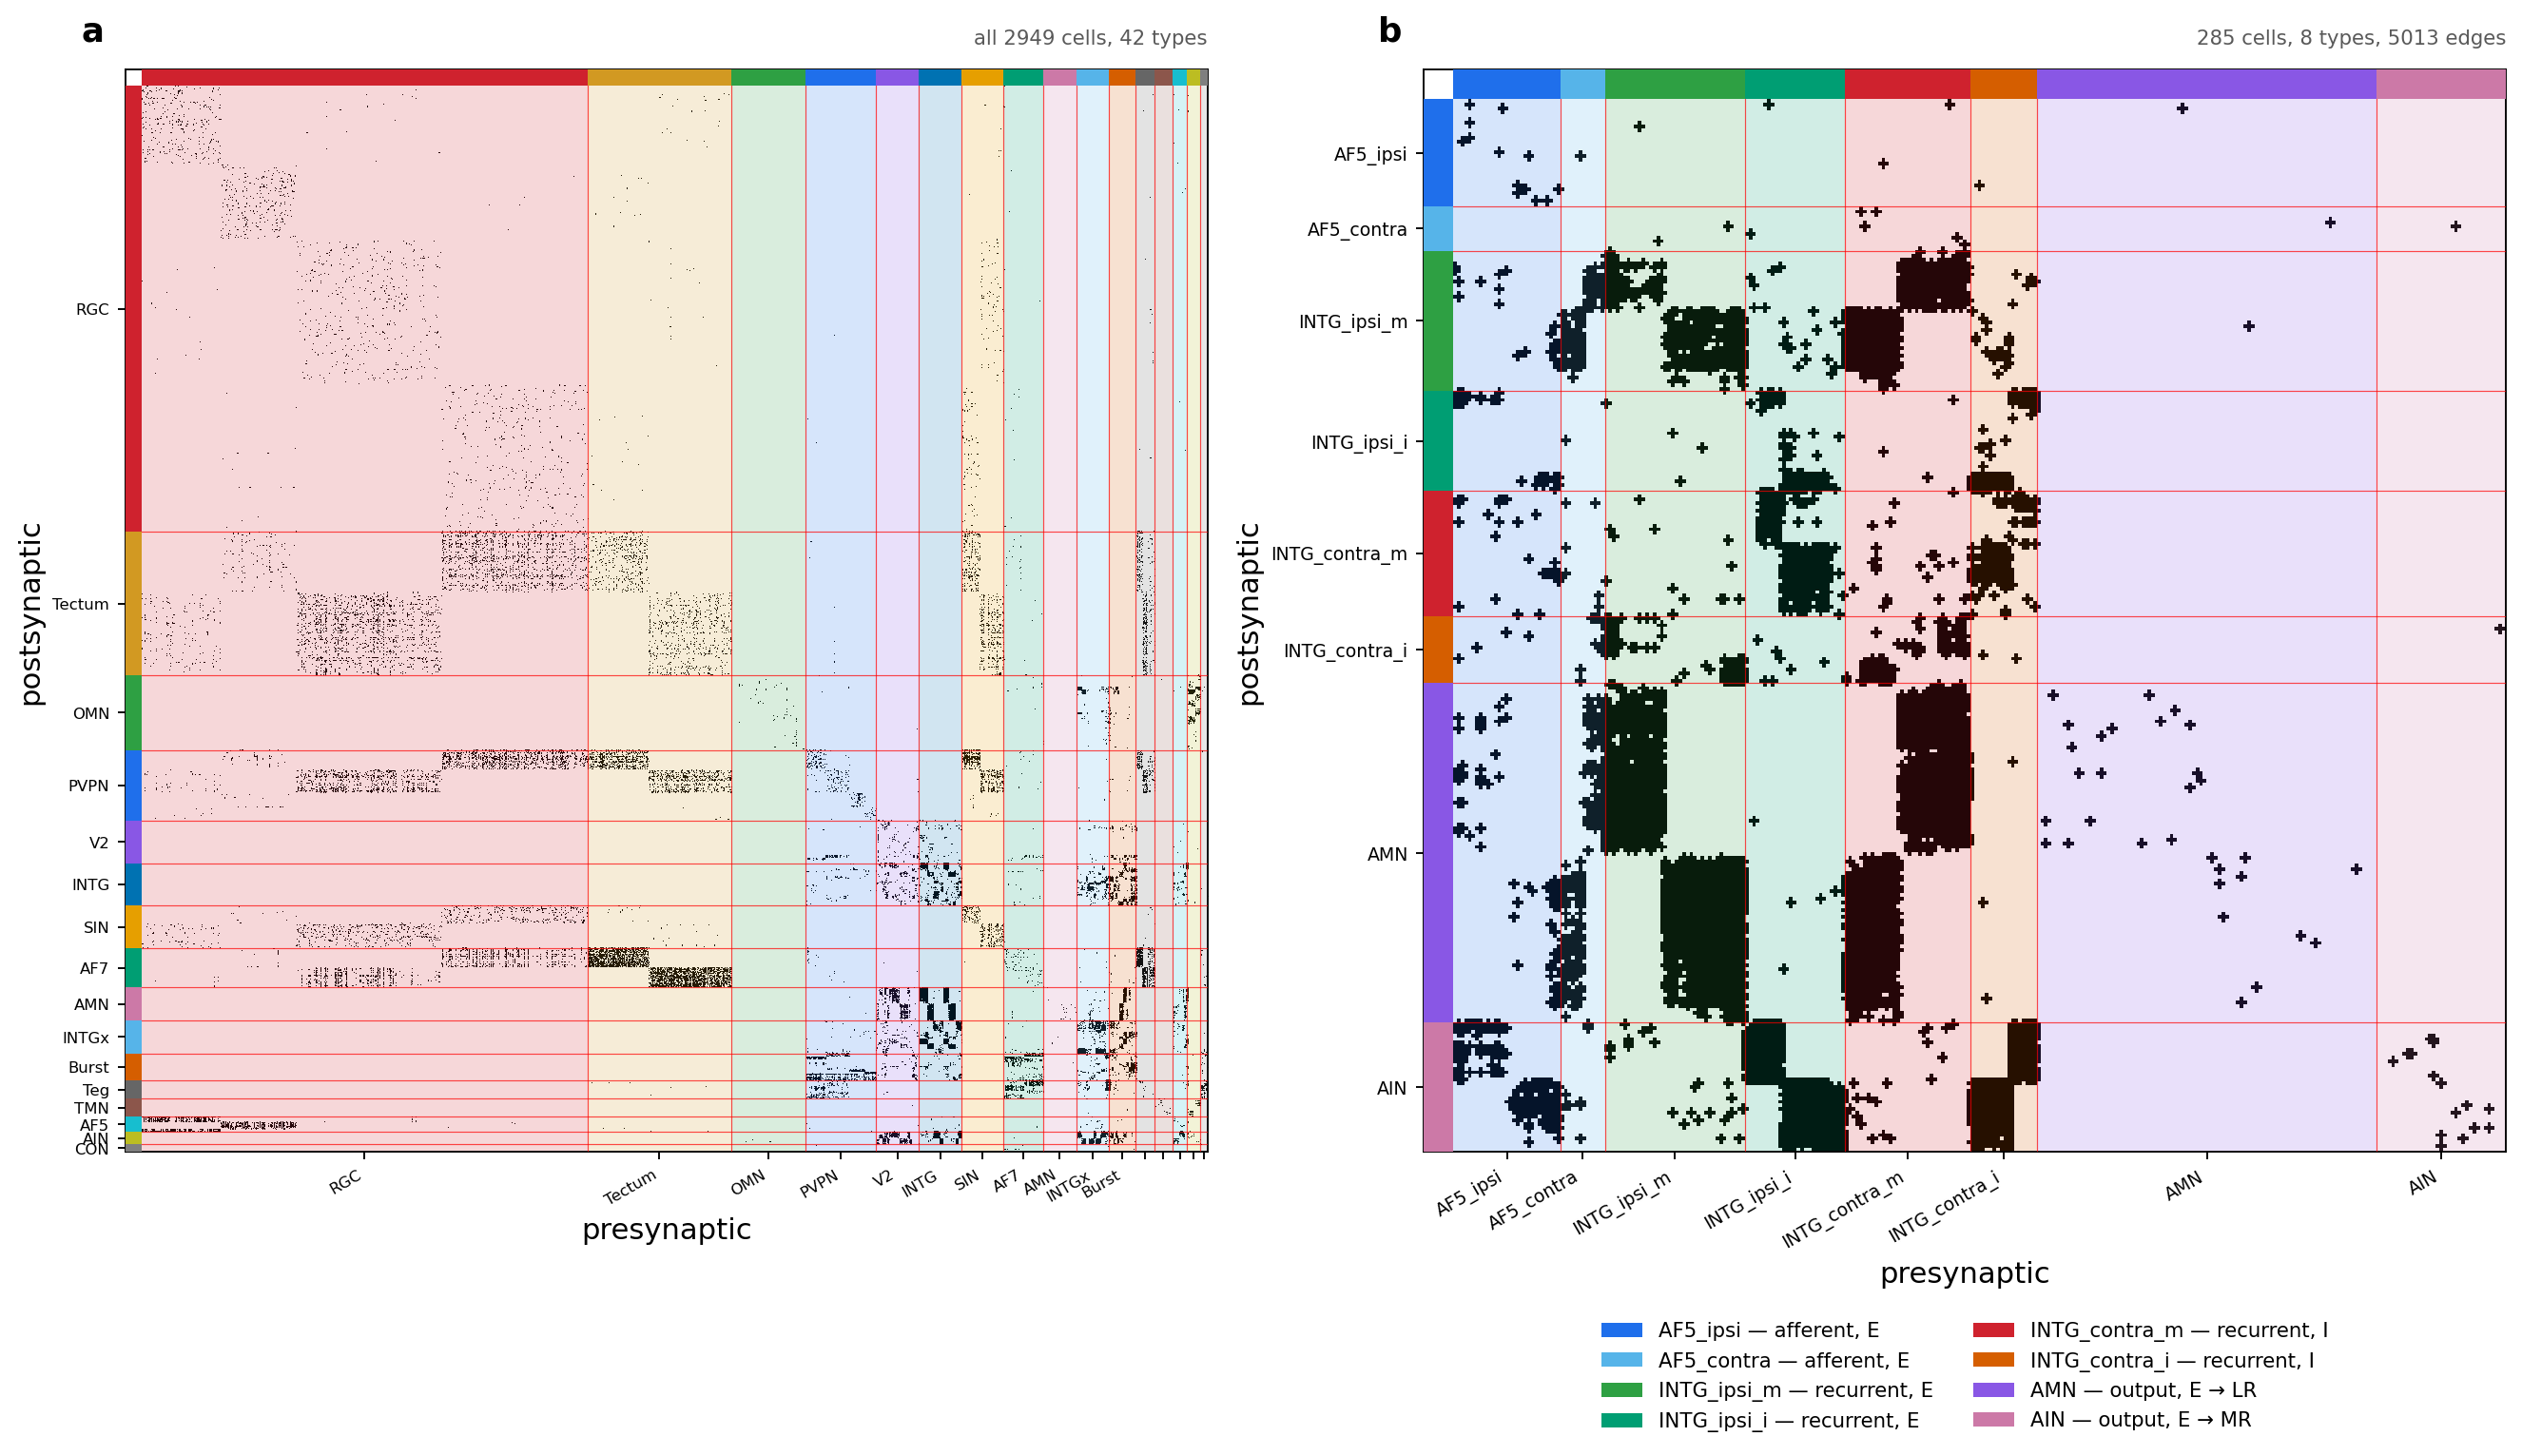
\includegraphics[width=\textwidth]{../figures/zebrafish/fig_oculomotor_circuit.png}
\caption*{\small \textbf{The oculomotor reconstruction and the sub-circuit modelled here.} (a) All 2949 cells, ordered by the 16 coarse cell-type families, support mask of the synapse-area matrix. (b) The 285-cell sub-circuit, ordered afferent then recurrent then output, and within a type left hemisphere before right. Colour carries the biology: blue = afferent, green = excitatory recurrent, red/orange = inhibitory recurrent, purple/pink = motor output. (c) The same sub-circuit signed by the Dale assignment of section 1.4 --- each synapse coloured by the sign of its \emph{presynaptic} cell, blue excitatory, red inhibitory, shade log-scaled in synaptic area. This is what the model multiplies, $\hat W_{ij} = |\hat S_{ij}|\,\mathrm{sign}(W^{\mathrm{con}}_{ij})$, and the support mask of (b) cannot show it. Because the sign belongs to the column, the panel reads as vertical bands: the two \texttt{INTG\_contra} types are a solid red block, and it is visibly the only inhibition the 285 cells contain. Rows are postsynaptic, columns presynaptic in all three. Regenerate with \texttt{python scripts/plot\_oculomotor\_connectome.py --config config/zebrafish/zebrafish\_om\_intg\_285\_v1.yaml --out figures/zebrafish/fig\_oculomotor\_circuit.png}.}
\end{figure}

\begin{figure}[H]\centering
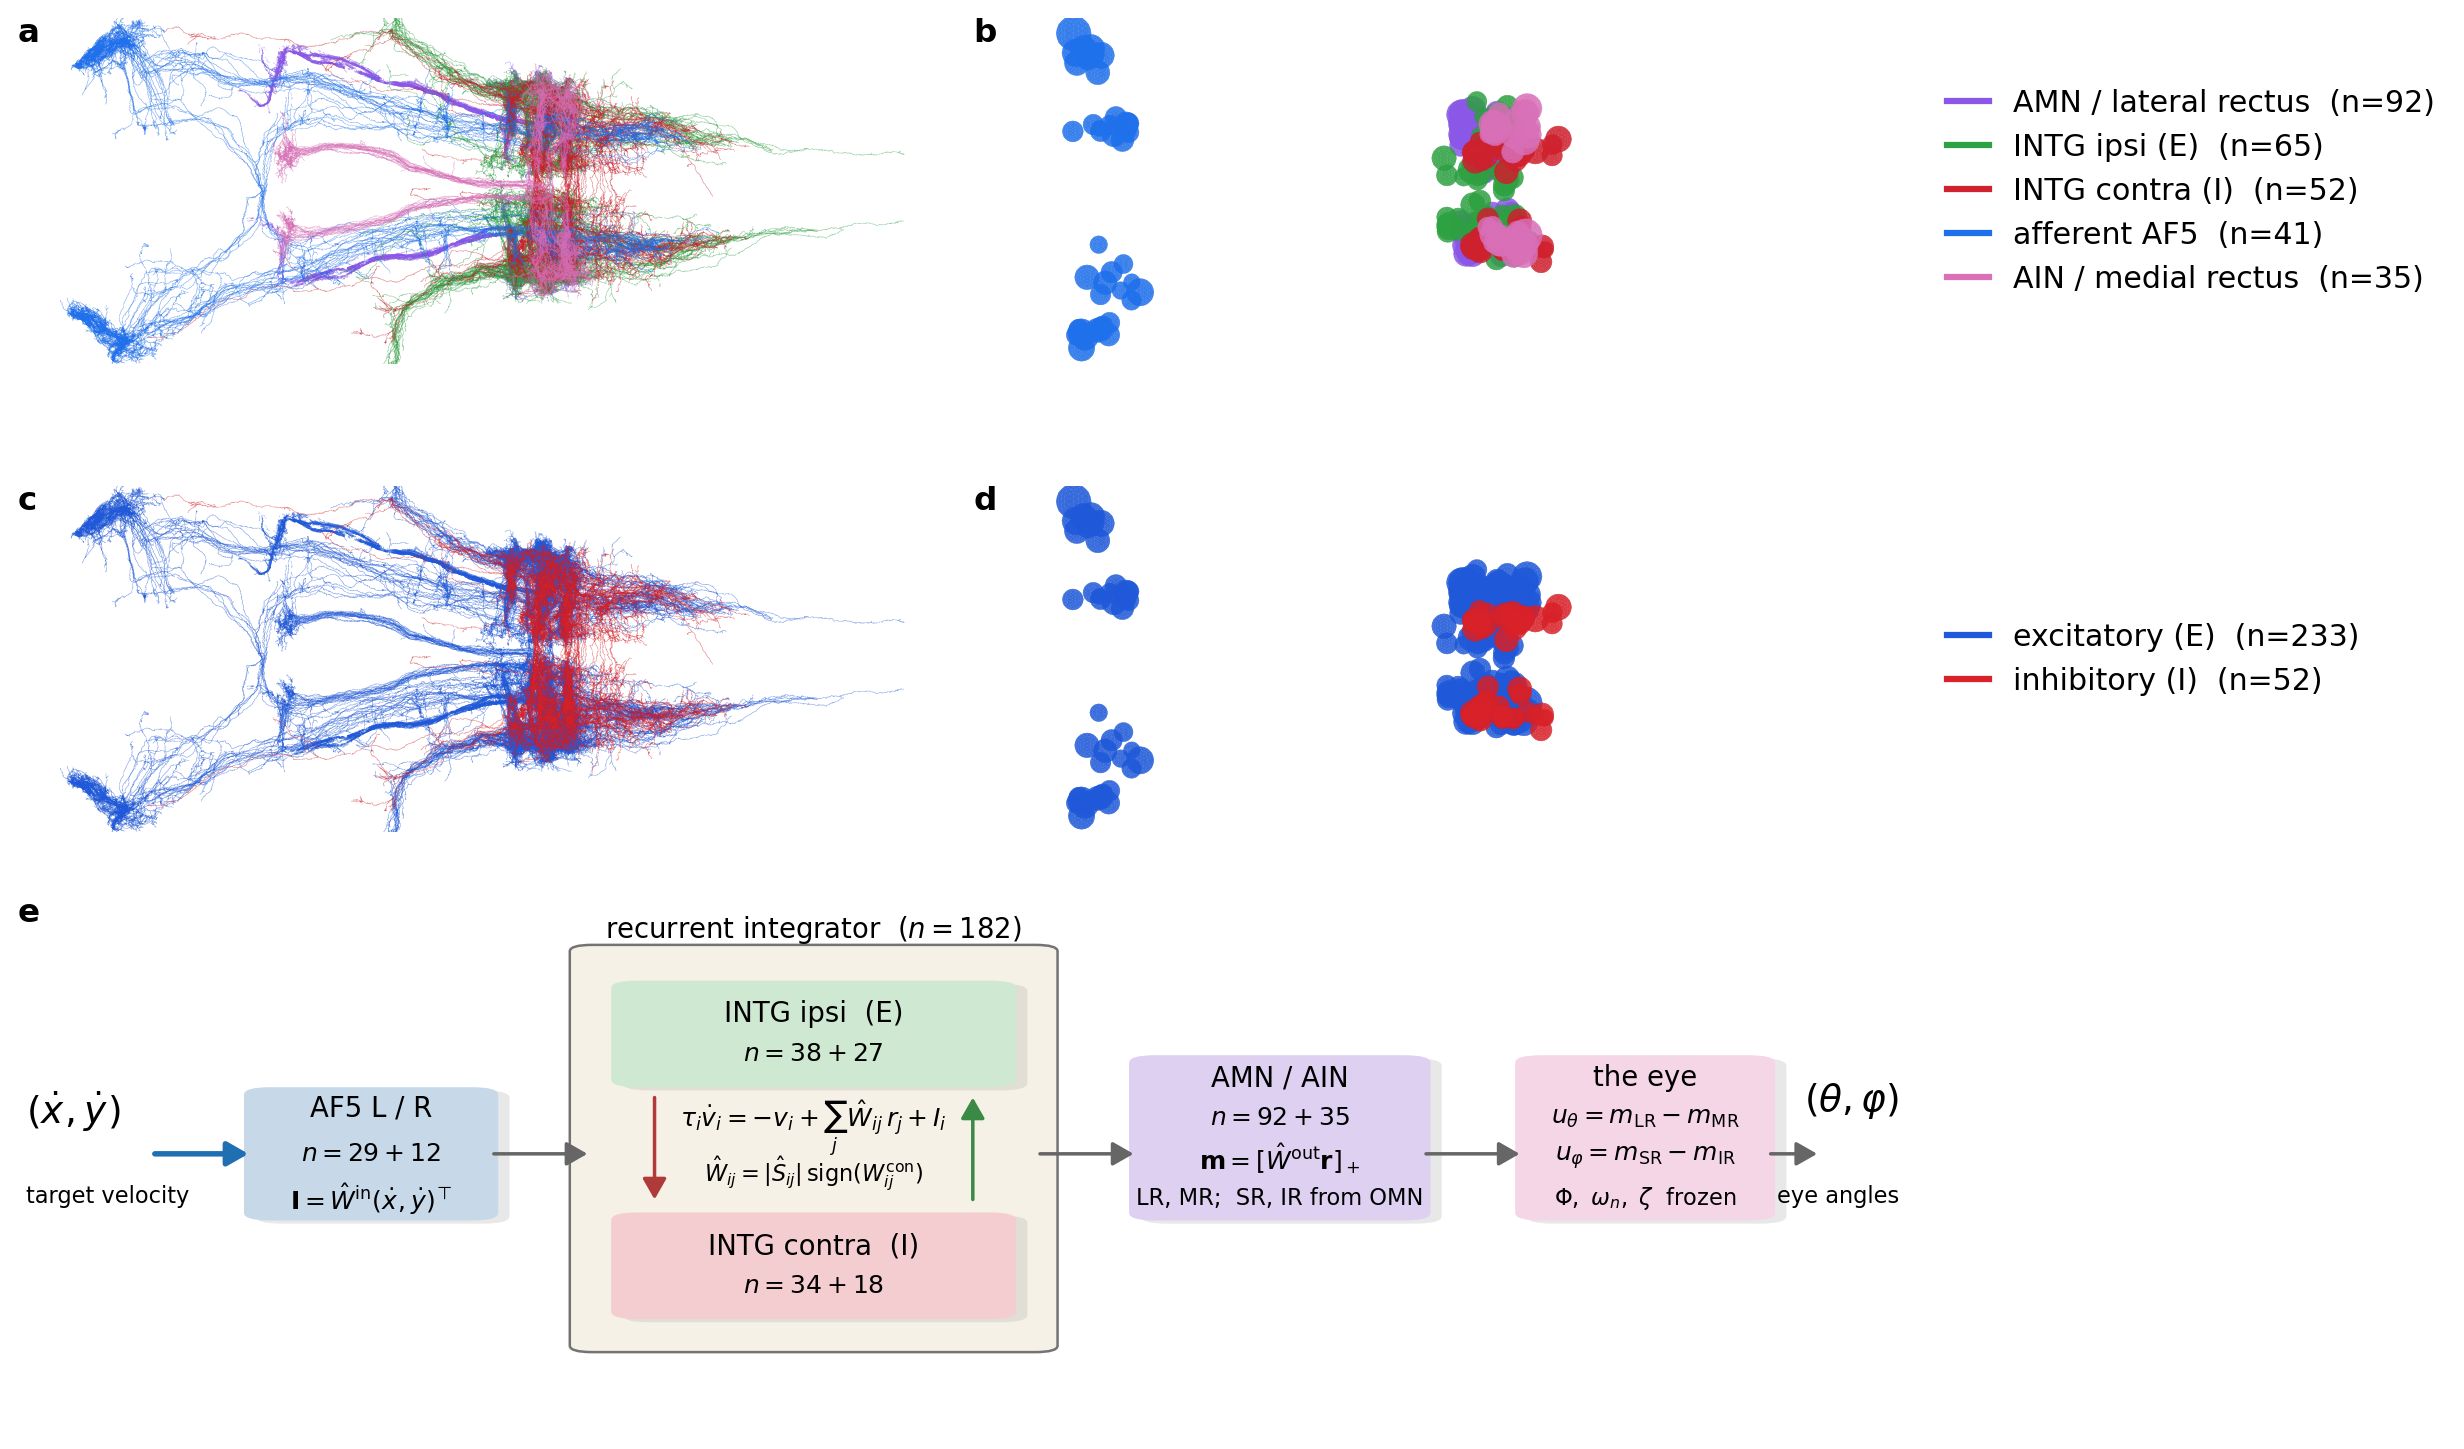
\includegraphics[width=\textwidth]{../figures/zebrafish/fig_1_oculomotor_overview.png}
\caption*{\small \textbf{Figure 1 --- the oculomotor circuit.} Twin of Figure 1 of the zebrafish heading-direction paper, rendered through the same code with the content swapped. \textbf{(a)} All 285 skeletons from the neuprint-fish2 reconstruction, dorsal view, coloured by role: AF5 afferents blue, ipsilateral (excitatory) INTG green, contralateral (inhibitory) INTG red, AMN purple, AIN pink. \textbf{(b)} The cell bodies alone, same view --- the AF5 somas sit well anterior of the integrator/motor cluster (radii scaled x0.3 for legibility, not a measurement). \textbf{(c, d)} The same skeletons and somas recoloured by Dale sign: blue excitatory (233 cells), red inhibitory (52 cells). The inhibitory population is exactly the contralateral integrator of section 1.4, and the two rows together are the claim being made --- that the E/I split is by projection laterality, not by anatomical position. \textbf{(e)} The computation of section 4 end to end: the target velocity $(\dot x,\dot y)$ enters through $\hat W^{\mathrm{in}}$ on the AF5 afferents, the INTG pool integrates under sign-locked continuous-time rate dynamics with mutual inhibition across the midline, $\hat W^{\mathrm{out}}$ reads non-negative motor drives, and the push-pull differences $u_\theta,u_\varphi$ drive the eye to the gaze angles $(\theta,\varphi)$. LR and MR have a pool in these 285 cells; SR and IR would come from OMN, which section 1.5 leaves out. Regenerate with \texttt{python figures/zebrafish/fig\_1\_oculomotor\_overview.py}.}
\end{figure}

\subsection*{1. The circuit}

\subsubsection*{1.1 Three pools}

Anatomy for all 285 cells was fetched from neuprint-fish2 and is shown in Figure 1. It had to be keyed on bodyId rather than cell type: the server does not carry the reconstruction's type names --- \texttt{INTG\_ipsi\_m} is \texttt{INTGip1} there, \texttt{INTG\_contra\_m} is \texttt{INTGco1} --- and the two AF5 populations carry no type at all, so a type query returns 142 of 285 cells and drops the whole afferent stage. All 285 bodyIds resolve.

The 285 cells divide into an input stage, a recurrent integrator and a motor output stage.

\begin{center}\small
\begin{tabularx}{\textwidth}{>{\raggedright\arraybackslash}X>{\raggedright\arraybackslash}X>{\raggedright\arraybackslash}X>{\raggedright\arraybackslash}X}\toprule
pool & types & cells & Dale sign \\\midrule
afferent & \texttt{AF5\_ipsi} (29), \texttt{AF5\_contra} (12) & 41 & excitatory \\
recurrent & \texttt{INTG\_ipsi\_m} (38), \texttt{INTG\_ipsi\_i} (27), \texttt{INTG\_contra\_m} (34), \texttt{INTG\_contra\_i} (18) & 117 & ipsi excitatory, contra inhibitory \\
output & \texttt{AMN} (92), \texttt{AIN} (35) & 127 & excitatory \\
\bottomrule\end{tabularx}\end{center}

Within the sub-circuit there are 5013 edges, a density of 6.2 \% --- an order of magnitude above the 0.51 \% of the full reconstruction. That concentration is what one expects of a recurrent integrator core plus its dedicated input and output stages, and it is the first (weak) evidence that the selection is a circuit rather than an arbitrary subset.

\subsubsection*{1.2 AF5 is an afferent, and the wiring says so}

The two AF5 populations are the pretectal arborization field that carries optokinetic drive. Their afferent status is not assumed. In the measured matrix, AF5 sends 88.2 \% of its outgoing synaptic area into the INTG/AMN/AIN core and receives 1/178th as much back (6.89e5 out against 3.87e3 in). This is the same asymmetry test that confirmed the matrix orientation using the retinal ganglion cells, which are 15.4x more outgoing than incoming.

Both AF5 types are left/right balanced --- \texttt{AF5\_ipsi} 15 L / 14 R, \texttt{AF5\_contra} 6 L / 6 R --- so a bilateral input gate is expressible. This is worth stating because it is not generally true in this dataset: \texttt{RGC\_AF7} is reconstructed in the left hemisphere only (804 L / 0 R) and could not support a symmetric gate.

\subsubsection*{1.3 What drives the afferents --- CLAIM, and an open one}

The direction selectivity below is the circuit owner's description, not a measurement in this file. The combination rule is explicitly unresolved.

\begin{itemize}\setlength{\itemsep}{1pt}
  \item \textbf{\texttt{AF5\_ipsi}} --- the left pool is driven by rightward-eye motion that is leftward and/or forward; the right pool by leftward-eye motion that is rightward and/or forward.
  \item \textbf{\texttt{AF5\_contra}} --- the left pool is driven by rightward-eye motion that is rightward and/or backward; the right pool by leftward-eye motion that is leftward and/or backward.
\end{itemize}

Whether the two conditions combine as AND, OR or XOR is \textbf{not known}. This is not a detail to be settled by a default: it decides whether a single afferent unit reports a conjunction (a narrow direction tuning) or a disjunction (a broad one), and therefore how much of the direction computation the recurrent circuit has to do itself. Until it is resolved, the input model should carry it as an explicit switch and the three variants should be trained and compared.

\subsubsection*{1.4 The integrator, and why the E/I split is by laterality}

The four INTG types are the velocity-to-position integrator. The sign assignment follows their projection laterality: \textbf{ipsilateral projections excitatory, contralateral projections inhibitory}. That is the classical integrator motif --- two half-integrators, one per hemisphere, each self-exciting locally and inhibiting its opposite number across the midline. Mutual inhibition is what lets the pair hold a \emph{signed} position variable on a single positive-rate substrate. Panels (c) and (d) of Figure 1 plot the assignment on the anatomy --- blue excitatory, red inhibitory --- and what they show is that it is not readable from position: the 52 inhibitory cells are interdigitated with the 233 excitatory ones in the same hindbrain column, which is why the split has to be asserted per cell type rather than inferred from where a soma sits.

This is a Dale assignment by cell type, exactly as in the heading-direction circuit, where \texttt{\_ZHD\_INH\_PREFIXES} in \texttt{connectome\_loaders.py} encodes the claim that the r1pi/dIPN cells are GABAergic. Neither is a measurement. The difference is that here the claim is written in the config, per type, where it can be reviewed and flipped, rather than in a tuple of string prefixes inside a loader.

\subsubsection*{1.5 The output stage, and one simplification worth flagging}

Only the \textbf{horizontal} pair of extraocular muscles is modelled:

Throughout, \textbf{the eye} means everything downstream of the last neuron --- the globe, its six muscles, the orbital tissue and their mechanics. What matters is the boundary rather than the word: the circuit's output is a muscle command, the eye turns that command into an angle, and the eye is measured and frozen while the circuit is learned. The engineering literature, and several of the sources cited later, call this the \emph{plant}; it is the same thing. Section 5.1 identifies it.

\begin{itemize}\setlength{\itemsep}{1pt}
  \item \texttt{AMN} drives the \textbf{lateral rectus} (\texttt{LR} in the eye model), which abducts the eye;
  \item \texttt{AIN} drives the \textbf{medial rectus} (\texttt{MR}), which adducts it.
\end{itemize}

Muscle keys refer to the six-muscle soft-body eye in \texttt{Plexus/prototype/eye}, where each muscle carries an innervation state \texttt{muscle.act} and the globe's pose is recovered by a Kabsch fit (\texttt{eye\_pose} -> horizontal, vertical, torsion in degrees). Coupling the readout to that eye, rather than to an abstract scalar, is what would make "eye position" a mechanical quantity instead of a fitted one.

\textbf{The simplification.} \texttt{AIN} are abducens \emph{internuclear} neurons. In vivo they are not motor neurons: they project across the midline to the oculomotor nucleus (\texttt{OMN}), whose motor neurons innervate the medial rectus. \texttt{OMN} is 207 cells in this reconstruction and is \textbf{not} in the selected pool. Treating \texttt{AIN} as driving the medial rectus therefore collapses a two-synapse pathway into one, and drops the sign inversion and delay that the missing synapse would contribute. This is a legitimate modelling choice, but it should be stated in any write-up, and the obvious control is to add \texttt{OMN} to \texttt{circuit.cell\_types} and check whether the fitted dynamics change.

\subsubsection*{1.6 What is not in the pool}

Two omissions are deliberate and one of them constrains the task:

\begin{itemize}\setlength{\itemsep}{1pt}
  \item \textbf{\texttt{Burst\_T1A/T1B/T8/T9/T10}} (74 cells) are the saccadic burst generators --- the source of the brief velocity command that a saccadic integrator integrates. They are excluded, so in the current pool the only anatomically defined input is the optokinetic AF5 drive. A saccade-driven task would have to inject velocity directly into INTG, which is a modelling choice, not a connectome-derived pathway.
  \item \textbf{\texttt{OMN}} (207 cells), as described in \S{}1.5.
\end{itemize}

\subsection*{2. The task}

\subsubsection*{2.1 What the network computes}

The oculomotor integrator converts an eye-\textbf{velocity} command into an eye- \textbf{position} command: the motor neurons must hold a rate proportional to position long after the velocity signal has gone. Written as the leaky integral of the drive, per axis,

\begin{equation*}
\frac{d\theta}{dt} = -\frac{\theta}{\tau} + s_\theta\,\dot x(t),
\qquad
\frac{d\varphi}{dt} = -\frac{\varphi}{\tau} + s_\varphi\,\dot y(t)
\end{equation*}

where $(\theta,\varphi)$ are the horizontal and vertical eye angles and $(\dot x,\dot y)$ the target velocity --- the notation of section 4, in which $v$ is reserved for membrane voltage. The quantity of interest is $\tau$, the time constant over which eye position leaks back to centre. A perfect integrator is $\tau = \infty$; the biological integrator is finite, and measuring what $\tau$ the connectome-constrained circuit can support is the point of the exercise.

\subsubsection*{2.2 Saccades versus optokinetic drive}

The two natural stimulus regimes differ, and the choice interacts with \S{}1.6:

\begin{itemize}\setlength{\itemsep}{1pt}
  \item \textbf{Optokinetic}: sustained whole-field motion, the drive AF5 actually carries. Slow, continuous velocity --- the regime the selected pool supports anatomically.
  \item \textbf{Saccadic}: brief high-velocity pulses separated by fixations, the classical integrator probe. This is the regime the burst generators serve, and they are not in the pool.
\end{itemize}

The swim generator's stimulus is a Poisson train of boxcar impulses (\texttt{swim\_rate\_hz}, \texttt{swim\_duration\_s}) --- structurally a saccade train already. So the saccadic regime is reachable by reparameterising the existing generator rather than writing a new one; what is missing is anatomy for the input, not code.

\subsubsection*{2.3 The open-loop problem}

Coarsely: the circuit is asked to keep a moving target centred on the fovea while being told only how fast the target is moving, never where it is. That is the situation the anatomy puts it in. AF5 is a motion-sensitive arborization field --- it reports optokinetic \emph{velocity} --- and nothing in the selected 285-cell pool reports absolute target position. A controller with position feedback can always correct, so its errors do not accumulate; a controller given velocity alone must reconstruct position by integration and has nothing to check the result against. Drift is therefore not a failure of the circuit but a property of the problem, and the meaningful question is not whether the target is held but for how long.

More specifically, take the horizontal axis and write the target eccentricity $\theta^{\star}(t)$, the gaze $\theta(t)$, and the retinal error $\varepsilon = \theta^{\star} - \theta$; the vertical axis is the same with $\varphi$. Every trial starts foveated at the centre, $\theta(0)=\theta^{\star}(0)=0$. The eye here is idealised as rate control: the motor command sets gaze \emph{velocity}, so gaze angle is its integral. The ideal controller is then

\begin{equation*}
\frac{d\theta}{dt} = \dot\theta^{\star}(t) = s_\theta\,\dot x(t)
\qquad\Longrightarrow\qquad
\varepsilon(t) = 0 \ \ \forall\, t
\end{equation*}

and tracking is exact. The interesting cases are the three ways a biological integrator departs from it, each of which produces a different growth law for $|\varepsilon|$ --- which is what makes them separable from a single measured trace.

\textbf{Gain.} If the velocity-to-position conversion is miscalibrated by a factor $k$,

\begin{equation*}
\frac{d\theta}{dt} = k\,\dot\theta^{\star}(t)
\qquad\Longrightarrow\qquad
\varepsilon(t) = (1-k)\,\big[\theta^{\star}(t)-\theta^{\star}(0)\big]
\end{equation*}

The error is proportional to the \emph{displacement} from the start, not to the distance travelled, because integration is linear. In a bounded workspace displacement is capped by the arena, so this error is self-limiting: in our geometry the target reaches a median 1.16 arena units from the centre, and $|1-k|$ must exceed 0.52 before the target can leave a 0.6-unit fovea at all. A realistic miscalibration of a few percent is invisible. Gain is not what loses the target.

\textbf{Leak.} A real integrator is imperfect and relaxes toward its rest state with a time constant $\tau$:

\begin{equation*}
\frac{d\theta}{dt} = -\frac{\theta}{\tau} + \dot\theta^{\star}(t)
\end{equation*}

In the frequency domain this is a \emph{high-pass} on target eccentricity, corner frequency $1/\tau$. Sustained excursions are under-represented, so the error saturates rather than growing without bound, and gaze is a shrunken, centre-biased copy of the truth. The counterintuitive consequence is that \emph{slow} targets are lost first, because their motion is exactly the low-frequency content the leak removes. Measured: at $\tau = 2$ s a fast target is never lost within 20 s while a slow one goes at 5.9 s, and the slow case needs $\tau \geq 8$ s to survive. $\tau$ is the quantity the INTG pool exists to make long, and this is the curve that says how long is long enough.

\textbf{Noise.} If the integrated velocity carries a white perturbation of intensity $\sigma$,

\begin{equation*}
\frac{d\theta}{dt} = \dot\theta^{\star}(t) + \sigma\,\xi(t),
\qquad \langle \xi(t)\,\xi(t')\rangle = \delta(t-t')
\end{equation*}

the error is a random walk: $\mathrm{std}[\varepsilon(T)] = \sigma\sqrt{T}$ per axis, unbounded but with zero mean. It is the only one of the three that cannot be corrected by better calibration and the only one that averages away across trials, so it is invisible to any analysis that pools trials before measuring drift.

Three growth laws --- bounded-linear, saturating, and square-root --- over one shared quantity. A drift trace measured from the real circuit can therefore be \emph{classified}, not merely reported, which is the point of setting the problem up this way. \texttt{prototype/dot\_tracking/openloop.py} implements the gain and leak cases and measures the survival time \texttt{t\_lose}, the first moment $|\varepsilon|$ exceeds the fovea; the noise case is stated here for completeness but is not in the prototype, since a zero-mean drift is better measured against recorded data than against a simulation of itself.

\subsection*{3. The training dataset}

\subsubsection*{3.1 Where it comes from}

Task data is generated by \texttt{GNN\_Main.py -o generate <config>}, which reaches \texttt{data\_generate} -> \texttt{data\_generate\_task} (dispatch on \texttt{task.task\_type}) -> \texttt{\_generate\_swim\_integration\_task}, all in \texttt{src/connectome\_gnn/generators/graph\_data\_generator.py}.

The critical property: \textbf{generation is connectome-agnostic}. The generator writes \texttt{stimulus.zarr} of shape (trials, T, channels) and \texttt{target.zarr} of shape (trials, T, columns) --- pure time series, with no notion of a neuron. The circuit appears only as a \texttt{circuit\_provenance.json} written beside the splits, recording the circuit name, cell count and the SHA-256 of \texttt{J\_effective}, so a dataset can later be checked against the circuit a checkpoint was trained on.

The consequence for planning: the dataset can be generated and inspected \textbf{before} the circuit registry entry, the connectome CSVs or the E/I assignment exist. That is the cheapest next step on this branch.

\subsubsection*{3.2 Parameters that define it}

\begin{center}\small
\begin{tabularx}{\textwidth}{>{\raggedright\arraybackslash}X>{\raggedright\arraybackslash}X}\toprule
parameter & meaning \\\midrule
\texttt{n\_trials\_train} / \texttt{n\_trials\_test} & independent trials per split \\
\texttt{n\_steps}, \texttt{dt} & samples per trial and the timestep, so trial duration is \texttt{n\_steps * dt} \\
\texttt{swim\_rate\_hz} & mean Poisson rate of impulse onsets --- the saccade rate \\
\texttt{swim\_duration\_s} & boxcar width of one impulse --- the saccade duration \\
\texttt{forward\_vel\_mean} / \texttt{forward\_vel\_std} & amplitude distribution of the velocity drive \\
\texttt{target\_kind} & which target is assembled; \texttt{scalar\_xi} is the integrator \\
\texttt{xi\_tau\_s} & the leak; absent or <= 0 gives a perfect integrator \\
\texttt{seed} & stimulus RNG; fixed across baseline and comparison runs \\
\bottomrule\end{tabularx}\end{center}

\texttt{training.task\_targets} then projects the on-disk superset down to the columns a given run trains on, so one dataset serves several sub-tasks.

\subsection*{4. The whole model in one notation}

\begin{figure}[H]\centering
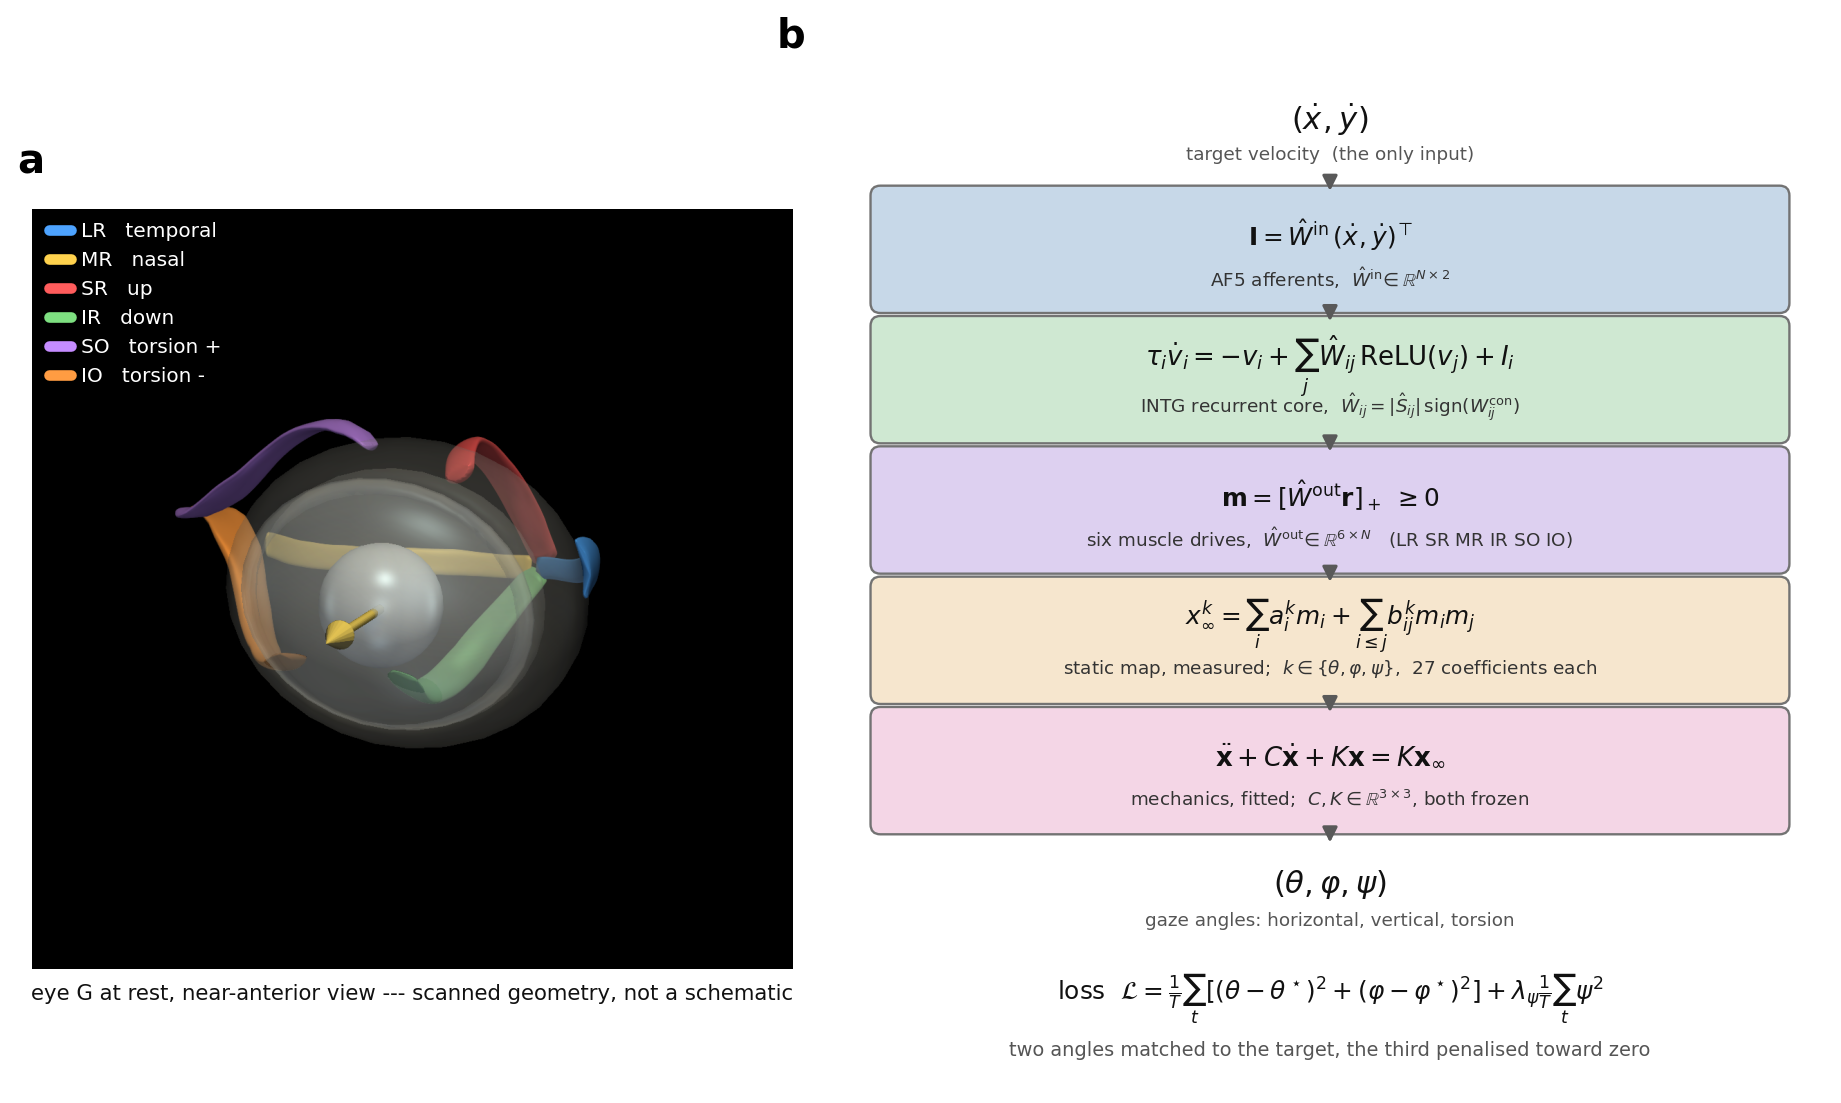
\includegraphics[width=\textwidth]{../figures/zebrafish/fig_eye_schematic.png}
\caption*{\small \textbf{The eye, and the symbols of the model.} \textbf{(a)} The globe seen down the corneal axis with the six extraocular muscles at their true insertions, drawn from \texttt{eye\_anatomy.MUSCLES} --- the same table the MPM uses to shape the straps, so this is the model's own geometry. Only the horizontal pair is innervated by this circuit: LR abducts (positive gaze), MR adducts. The four faint muscles exist in the eye but receive no command. The two axes the model uses are marked: horizontal gaze $\theta$, positive in abduction, and vertical gaze $\varphi$. \textbf{(b)} Every symbol of the nine steps below, in the order the signal meets them: the target velocity $(\dot x,\dot y)$, the input map $\hat W^{\mathrm{in}}$ onto the AF5 afferents, the sign-locked recurrent core, the output map $\hat W^{\mathrm{out}}$ onto four non-negative motor pools, the push-pull commands $u_\theta,u_\varphi$, the frozen per-axis eye, and the loss on the gaze angles $(\theta,\varphi)$ --- after the eye, not on the command. Regenerate with \texttt{python fit\_plant.py} and \texttt{python fig\_eye\_schematic.py} in \texttt{Plexus/prototype/eye}.}
\end{figure}


Written in the formalism of \texttt{neurips.tex}, with the symbols laid out in the figure above, so the oculomotor circuit and the flyvis work can be read side by side. Every stage from the two numbers the circuit is given to the two angles it is scored on is written out below, because the intermediate quantities are where the modelling choices are, and they are invisible in any summary that jumps from "velocity in" to "position out".

\begin{center}\small
\begin{tabularx}{\textwidth}{>{\raggedright\arraybackslash}X>{\raggedright\arraybackslash}X>{\raggedright\arraybackslash}X}\toprule
symbol & dimension & meaning \\\midrule
$x(t),\,y(t)$ & arena units & target position in the world \\
$\dot x(t),\,\dot y(t)$ & units s$^{-1}$ & target velocity --- \textbf{the only input} \\
$s_\theta,\,s_\varphi$ & deg / unit & world-to-angle scale, one per axis \\
$\theta^{\star},\,\varphi^{\star}$ & deg & target eccentricity, horizontal and vertical \\
$v_i(t)$ & --- & membrane voltage of neuron $i$ ($N=285$) \\
$\tau_i$ & s & membrane time constant of neuron $i$ \\
$r_i(t)$ & --- & firing rate, $r_i=\rho(v_i)$ \\
$\hat W \in \mathbb{R}^{N\times N}$ & --- & recurrent weights, sign-locked to the connectome \\
$\hat W^{\mathrm{in}} \in \mathbb{R}^{N\times 2}$ & --- & velocity to afferents; rows zero outside AF5 \\
$\hat W^{\mathrm{out}} \in \mathbb{R}^{4\times N}$ & --- & rates to muscles; columns zero outside the motor pools \\
$m_{\mathrm{LR}},m_{\mathrm{MR}},m_{\mathrm{SR}},m_{\mathrm{IR}}$ & $\ge 0$ & motor-pool drives, one per muscle \\
$u_\theta,\,u_\varphi$ & $[-1,1]$ & push-pull commands, one per axis \\
$\Phi_\theta,\,\Phi_\varphi$ & deg & static nonlinearity of the eye, per axis \\
$\omega_n,\,\zeta$ & rad s$^{-1}$, --- & eye mechanics, per axis \\
$\theta(t),\,\varphi(t)$ & deg & \textbf{eye angles} --- horizontal and vertical gaze \\
\bottomrule\end{tabularx}\end{center}

A hat marks a learned quantity. $v$ is the membrane voltage throughout and never a velocity; the velocities are $\dot x$ and $\dot y$, and the eye's orientation is the pair $(\theta,\varphi)$, horizontal first.

\textbf{Step 0 --- the world sets the angles.} The target moves in a bounded arena in units, and each axis is mapped to degrees by its own scale, because the eye's reachable travel is not the same horizontally and vertically (section 4.2):

\begin{equation*}
\theta^{\star}(t) = s_\theta\, x(t),
\qquad
\varphi^{\star}(t) = s_\varphi\, y(t),
\qquad
\theta^{\star}(0)=\varphi^{\star}(0)=0
\end{equation*}

\textbf{Step 1 --- what the circuit is given.} Only the velocity, never the position. This is the open-loop premise of section 2.3 written as a vector:

\begin{equation*}
\mathbf{u}(t) \;=\; \big(\dot x(t),\ \dot y(t)\big)^{\!\top} \in \mathbb{R}^{2}
\end{equation*}

\textbf{Step 2 --- the input map $\hat W^{\mathrm{in}}$.} The drive enters only through the AF5 afferents $\mathcal{A}$ ($|\mathcal{A}|=41$). That restriction is the whole content of "connectome-constrained input": a free input layer would let the optimiser inject velocity wherever it is most convenient, which is exactly the degree of freedom the anatomy is supposed to remove:

\begin{equation*}
\mathbf{I}(t) \;=\; \hat W^{\mathrm{in}}\,\mathbf{u}(t),
\qquad
\hat W^{\mathrm{in}}_{i,:} = \mathbf{0}\ \ \ \forall\, i\notin\mathcal{A},
\qquad \mathcal{A}=\mathcal{A}_{\mathrm{AF5}}^{L}\cup\mathcal{A}_{\mathrm{AF5}}^{R}
\end{equation*}

so $\hat W^{\mathrm{in}}$ is $285\times 2$ with $41\times 2 = 82$ free entries out of 570. Componentwise, neuron $i$ receives $I_i = \hat W^{\mathrm{in}}_{i1}\dot x + \hat W^{\mathrm{in}}_{i2}\dot y$, and the direction tuning of section 1.3 --- still a CLAIM --- is what says whether that row should be free or fixed to a preferred direction.

\textbf{Step 3 --- the circuit.} The $N=285$ neurons obey the same rate equation as Eq. (1) of \texttt{neurips.tex}:

\begin{equation*}
\tau_i\frac{d v_i(t)}{dt} \;=\; -\,v_i(t) \;+\; V_i^{\mathrm{rest}}
\;+\!\!\sum_{j\in\mathcal{N}_i}\!\! \hat{W}_{ij}\,r_j(t)
\;+\; I_i(t) \;+\; \sigma\,\xi_i(t),
\qquad r_j=\rho(v_j)
\end{equation*}

with $\mathcal{N}_i$ the presynaptic partners of $i$ and $\rho$ the rate nonlinearity --- $\mathrm{ReLU}$ in the constrained model, $\tanh$ in the prototype of section 5.

\textbf{Step 4 --- the sign lock.} Only the magnitudes are learned; the signs are the measured Dale assignment of section 1.4, plotted in panels (c) and (d) of Figure 1, so $\hat W$ never leaves the connectome's sign pattern:

\begin{align*}
\hat{W}_{ij} \;=\; \big|\hat{S}_{ij}\big|\;\mathrm{sign}\big(W^{\mathrm{con}}_{ij}\big),
\qquad
\mathrm{sign}\big(W^{\mathrm{con}}_{ij}\big)=
\begin{cases}
-1, & j\in\mathcal{I} \quad(\text{INTG contra, } 52 \text{ cells})\\[2pt]
+1, & \text{otherwise} \quad(233 \text{ cells})
\end{cases}
\end{align*}

\textbf{Step 5 --- the output map $\hat W^{\mathrm{out}}$.} The motor pools are read as non-negative drives, one per muscle, ordered LR, MR, SR, IR:

\begin{equation*}
\mathbf{m}(t) \;=\; \big[\,\hat W^{\mathrm{out}}\mathbf{r}(t)\,\big]_{+}
\;=\;\big(m_{\mathrm{LR}},\,m_{\mathrm{MR}},\,m_{\mathrm{SR}},\,m_{\mathrm{IR}}\big)^{\!\top},
\qquad
\hat W^{\mathrm{out}}_{:,i} = \mathbf{0}\ \ \ \forall\, i\notin\mathcal{M}
\end{equation*}

with $[\cdot]_+$ a rectifier ($\mathrm{softplus}$ in the prototype) enforcing $m_\bullet\ge 0$, and $\mathcal{M}$ the motor pool. In the selected 285 cells $\mathcal{M}$ is AMN (92 cells, row LR) and AIN (35 cells, row MR) only, so $\hat W^{\mathrm{out}}$ is $4\times285$ with two live rows and $127$ live columns. \textbf{The vertical pair has no anatomical pool here}: SR and IR are innervated by OMN, which section 1.5 leaves out of the selection. The two-axis form is written because the eye and the prototype are two-axis; the constrained circuit as currently scoped commands $\theta$ alone, and reaching $\varphi$ means adding OMN to \texttt{circuit.cell\_types}.

\textbf{Step 6 --- push-pull.} Each axis is the difference of an antagonist pair, so a signed angle is carried on strictly non-negative rates by construction rather than by a free linear readout that might or might not discover it:

\begin{equation*}
u_\theta(t) = m_{\mathrm{LR}}(t) - m_{\mathrm{MR}}(t),
\qquad
u_\varphi(t) = m_{\mathrm{SR}}(t) - m_{\mathrm{IR}}(t)
\end{equation*}

\textbf{Step 7 --- the eye, per axis.} Each command drives a Hammerstein eye: a monotone static nonlinearity followed by second-order mechanics, with $\Phi$, $\omega_n$ and $\zeta$ identified in section 4.1 and \textbf{frozen} --- steps 6 and 7 together are what this note calls the \textbf{lateral-horizontal Hammerstein model}, and section 4.2 says what has to replace it --- registered as buffers, not parameters, because the body is measured and letting the optimiser retune it would defeat the point:

\begin{equation*}
\Phi_\theta(u_\theta)=a_\theta\,u_\theta + b_\theta\,u_\theta^{2},
\qquad
\ddot\theta+2\zeta_\theta\omega_\theta\,\dot\theta+\omega_\theta^{2}\,\theta
\;=\;\omega_\theta^{2}\,\Phi_\theta\big(u_\theta(t)\big)
\end{equation*}

\begin{equation*}
\Phi_\varphi(u_\varphi)=a_\varphi\,u_\varphi + b_\varphi\,u_\varphi^{2},
\qquad
\ddot\varphi+2\zeta_\varphi\omega_\varphi\,\dot\varphi+\omega_\varphi^{2}\,\varphi
\;=\;\omega_\varphi^{2}\,\Phi_\varphi\big(u_\varphi(t)\big)
\end{equation*}

The two axes have their own $(\Phi,\omega_n,\zeta)$, fitted from the LR/MR and the SR/IR probes separately; they differ by more than a factor of one and a half in travel, which is why $s_\theta \neq s_\varphi$ in step 0.

\textbf{Step 8 --- the objective.} Supervision is on the eye angles \emph{after} the eye, never on the command, in the same summed form as Eq. (3) of \texttt{neurips.tex}:

\begin{equation*}
\mathcal{L}_{\mathrm{pred}}=\sum_{t}
\Big\|\big(\theta(t),\varphi(t)\big)-\big(\theta^{\star}(t),\varphi^{\star}(t)\big)\Big\|_2
\end{equation*}

Putting the loss after the eye is what makes the network learn the eye's inverse rather than a velocity command: the gradient reaches $\hat W,\hat W^{\mathrm{in}},\hat W^{\mathrm{out}}$ through $\Phi$ and through the second-order mechanics, so a different eye trains a different controller. That is why section 4.2 lists one trained network per eye rather than one network tested on five.

\textbf{Step 9 --- discretisation and initial condition.} Forward Euler at $\Delta t = 1/60$ s, with the network state started at rest on every trial:

\begin{equation*}
v_i(t{+}\Delta t) = v_i(t) + \frac{\Delta t}{\tau_i}
\Big(-v_i(t) + \textstyle\sum_j \hat W_{ij} r_j(t) + I_i(t)\Big),
\qquad v_i(0)=0,\ \ \theta(0)=\varphi(0)=0
\end{equation*}

$v_i(0)=0$ has to \emph{mean} "eye centred", which is why every trajectory in the corpus starts at the centre (section 5.1). Nothing is carried between trials.

Two differences from the flyvis setting are worth naming. There the supervision is on $dv_i/dt$ of \emph{every} neuron, because the simulator provides the full state; here it is on two scalars at the far end of an eye, so the circuit is constrained only through its behavioural consequence. And there $\hat{W}$ is what is being recovered from activity, whereas here $\hat{W}$ is fixed in sign by the connectome and only its magnitudes, $\hat W^{\mathrm{in}}$ and $\hat W^{\mathrm{out}}$ are free. The oculomotor problem is thus the better-posed of the two: fewer unknowns, but a much narrower observation.

\textbf{What the trained controller of section 5 instantiates.} The same nine steps with the connectome removed, which is what makes the anatomy's cost measurable later: $N=64$ free units in place of the 285 cells, $\rho=\tanh$, $\hat W$ dense and initialised at zero with no sign lock, $\hat W^{\mathrm{in}}$ a dense $64\times2$ layer instead of 82 entries on AF5 rows, $\hat W^{\mathrm{out}}$ a dense $4\times64$ layer with all four muscle rows live. Steps 6 to 9 --- push-pull, the frozen per-axis eye, the loss on $(\theta,\varphi)$, the Euler step from $v=0$ --- are identical, so the gap between the two is attributable to the anatomy and to nothing else.

\subsubsection*{4.1 The eye model}

The circuit's output is muscle drive, not eye position, so the mechanics has to be in the loop --- and the MPM eye cannot be: its grid scatter is in-place, so it is not differentiable, and one trial costs more than all 7250 gradient updates of section 5.1. It is replaced by the reduced model of step 7, fitted by \texttt{fit\_plant.py} from the probe runs in \texttt{Plexus/prototype/eye/archive/}. Steps 6 and 7 together are the \textbf{lateral-horizontal Hammerstein model}: two antagonist pairs, two scalar commands, two independent single-input eyes.

Putting the whole nonlinearity in a memoryless block and leaving the dynamics linear is the \textbf{Hammerstein} structure --- the standard first move of block-oriented nonlinear system identification (Narendra and Gallman 1966; Bai 1998; Giri and Bai 2010), which dominates practice because it keeps the linear factor a transfer function, with every tool of linear systems theory intact, while the nonlinear factor stays a curve fitted pointwise. For an eye the split is anatomical rather than convenient: the nonlinearity is muscle and memoryless, the dynamics are globe and orbital tissue and near-linear at these rotations. It is also the classical oculomotor model --- Robinson (1964, 1981), with later work arguing the real eye carries more time scales than second order allows (Sklavos, Porrill, Kaneko and Dean, 2005).

The factorisation earns its keep here --- across mechanical configurations of the MPM eye the mechanics barely move, $\omega_n = 9.5$ to $11.1$ rad s$^{-1}$ and $\zeta = 0.22$ to $0.32$, while the static gain ranges over 14 to 23 degrees of travel. A configuration changes $\Phi$, not the ODE, so one set of dynamics covers a sweep. At $\zeta \approx 0.3$ the modelled eye is underdamped and rings at about 1.5 Hz; real eyes are overdamped, so that is a property of the MPM configuration rather than of a fish.

$\Phi$ and the mechanics are fitted \textbf{jointly}, against whole trajectories. The alternative --- read the plateaus for $\Phi$, then fit the transient --- needs settled plateaus, and this archive has none, for the reason given below.

\textbf{Second order wins, by about a factor of 3.} Against the first-order alternative $\tau\dot\theta + \theta = \Phi_\theta(u_\theta)$ --- viscosity and an elastic restoring force, no globe inertia --- the RMS error is 1.2--2.6 deg at first order against 0.41--0.77 at second, on every configuration that fits at all.

This is not a matter of degrees of freedom. A first-order system is monotone towards its target and \emph{cannot overshoot}, while the MPM eye overshoots and rings --- panel (b). Only the inertial term can produce that. And the fit has to be \textbf{per configuration}: pooled it gives RMS 5.05 deg and a static curve with plateaus at +16, +13 and +3 degrees for the same command; fitted separately, 0.41 to 0.77 deg.

\paragraph{What the eye does to a moving target}

In the prototype interface the red trace is $\Phi(u)$ --- where the eye \emph{would} settle if the command froze --- and the blue trace is where the eye actually is. At the speeds the task uses the two sit on top of each other, which looks as though the eye were doing nothing at all. It is not, and the reason is worth stating carefully, because it is the difference between an eye that distorts the command and one that merely postpones it.

Everything follows from the transfer function of step 7, the ratio of gaze to static command in the frequency domain:

\begin{equation*}
H(s)\;=\;\frac{\Theta(s)}{\Phi(s)}\;=\;\frac{\omega_n^{2}}
{s^{2}+2\zeta\omega_n s+\omega_n^{2}}
\end{equation*}

\textbf{It does not shrink the target.} $H(0)=1$ exactly, by construction. Hold any command and the eye ends up precisely at $\Phi(u)$ --- no steady-state error, no gain to calibrate away. This is the property that makes red and blue \emph{equal} rather than merely proportional.

\textbf{It delays it.} Expanding at low frequency,

\begin{equation*}
H(s)\;=\;1-\frac{2\zeta}{\omega_n}s+O(s^{2})\;\approx\;e^{-\Delta s},
\qquad
\Delta=\frac{2\zeta}{\omega_n}
\end{equation*}

which is a \textbf{pure time delay} to first order. Slow in, same thing out, $\Delta$ later. On the fitted eye that is 54 ms horizontally ($\zeta=0.263$, $\omega_n=9.76$ rad s$^{-1}$) and 40 ms vertically ($0.225$, $11.24$) --- about three frames at 60 Hz, which is why red sits on blue.

Measured on the simulator itself, by driving one axis with a small sinusoid and reading the phase, against the closed form above:

\begin{center}\small
\begin{tabular}{llll}\toprule
target & lag, horizontal & closed form & gain $\lvert$blue$\rvert/\lvert$red$\rvert$ \\\midrule
0.10 Hz & 54.0 ms & 54.0 & 1.003 \\
0.20 Hz & 54.6 ms & 54.6 & 1.014 \\
0.35 Hz & 56.3 ms & 56.4 & 1.043 \\
0.60 Hz & 61.6 ms & 62.1 & 1.135 \\
1.00 Hz & 81.1 ms & 83.3 & 1.445 \\
1.50 Hz & 143.9 ms & 152.5 & 1.935 \\
\bottomrule\end{tabular}\end{center}

Read it left to right. Below about 0.3 Hz the eye is a pure 54 ms delay at unity gain, and red and blue are the same curve shifted by three frames. Above that the delay grows and the gain \textbf{rises} --- rises, not falls, because $\zeta\approx0.26$ is underdamped, so the response peaks near $\omega_n/2\pi=1.55$ Hz at roughly

\begin{equation*}
\lvert H\rvert_{\max}\;\approx\;\frac{1}{2\zeta}\;=\;1.9
\end{equation*}

At 1.5 Hz the eye overshoots its own command by a factor of two. That amplification, not any lag, is what the small loops at direction reversals in the interface are: the command turns, the eye carries past it, and the two traces separate for as long as the ringing lasts.

Two consequences. For reading the interface, red on blue means the eye has caught up with its command, not that the eye is trivial --- the static map is still doing a factor of 15.3 degrees per unit of command, and the plot only looks tidy because it is drawn \emph{after} that map. For the task, the useful number is 0.3 Hz: below it the circuit can ignore the mechanics and solve a pure inversion of $\Phi$, above it the mechanics are part of the problem and the network has to learn a phase lead as well.

\emph{A correction.} An earlier note recorded the command leading the gaze by 0 ms at slow and middle speeds, from a cross-correlation. That was an artefact: the correlation peak of two smooth slow traces is flat across many frames, so the frame-quantised estimate collapsed to zero. Measured by single-frequency phase, the lag is 54 ms at every speed the task uses, and agrees with the closed form to a tenth of a millisecond.


\subsubsection*{4.2 Characterising the MPM eye}

The lateral-horizontal Hammerstein model of steps 6 and 7 assumes the eye is two independent axes driven by two signed scalars. The measurements say it is not. On eye G the superior oblique produces $+8.66$ degrees of torsion at full drive against $3.95$ of vertical, and the inferior oblique $-8.21$ against $2.88$: torsion is the \emph{largest} action of two of the six muscles. A model with no torsion coordinate cannot represent that, and a model with two commands cannot be told about it. This section is the replacement --- the model, the protocol that identifies it, and what eye G measured.

The aim is a procedure rather than a description of one eye. Something will replace eye G; nothing here should need re-deriving when it does. It is executable as \texttt{Plexus/prototype/eye/characterise\_eye.py}, and \texttt{PROTOCOL\_eye\_characterisation.md} beside it is the prose version.

\paragraph{The eye being characterised}

Eye G is an MLS-MPM eye whose geometry is \textbf{scanned rather than generated}: the globe and the six extraocular straps are filled with material points inside the meshes of a Blender reconstruction of a 96\,hpf larval head (\texttt{260802\_s2\_EYE\_MUSCLES\_MODEL.blend}), by the two seed operators \texttt{blend\_globe} and \texttt{blend\_muscles} of \texttt{blend\_mpm\_ops.py}. They are drop-in replacements for the analytic \texttt{eye\_anatomy} / \texttt{muscle\_morphogenesis} pair, so the rest of the plant --- pose readout, drive, contraction, socket, the shared grid --- is model F's mechanics unchanged. What changes is where the tissue is.

Two properties of that geometry matter for everything below, and both were measured rather than assumed. The \textbf{insertions are right}: driven in the four cardinal synergies the eye moves where the anatomy says it should, in all four (figure below, panel a). And the eye is \textbf{contact-limited rather than drive-limited}: scaling the globe by $1.2$ about its own centre buries the tendons in the sclera and costs $81\,\%$ of the temporal excursion, scaling it by $0.85$ collapses the nasal one from $8.5$ to $0.7$ degrees, and raising the drive $\times 1.5$ makes the globe lose $6.4\,\%$ of its radius and returns \texttt{NaN} strain. The working point is as hard as this geometry can be driven, which is why the workspace below is taken as given and characterised rather than tuned.

\paragraph{The shape of the model, coarsest first}

The eye takes six muscle drives and returns three angles:

\begin{equation}
\mathbf{m}(t)\in[0,1]^{6}
\;\longrightarrow\;
\mathbf{x}(t)=\big(\theta(t),\ \varphi(t),\ \psi(t)\big)\in\mathbb{R}^{3}
\label{eq:eye-io}
\end{equation}

horizontal, vertical and torsion, in degrees. The drives are one-sided because muscles pull and do not push, which is why they are not the signed $u_\theta,u_\varphi$ of step 6.

The single structural assumption is that the eye is a \textbf{static map followed by linear mechanics}. Where the eye eventually comes to rest is a nonlinear function of the drives; how it gets there is linear:

\begin{equation}
\mathbf{x}_{\infty}=g(\mathbf{m}),
\qquad
\ddot{\mathbf{x}}+C\,\dot{\mathbf{x}}+K\,\mathbf{x}=K\,\mathbf{x}_{\infty}
\label{eq:hammerstein}
\end{equation}

Hold the muscles at a fixed activation and the eye settles somewhere --- that is $g$. Change the activation and the globe swings to the new resting place with an overshoot and a ring --- that is $C$ and $K$. It is the factorisation of section 4.1 widened from one input and one angle to six and three, and it is what makes the thing measurable: $g$ is memoryless, so \textbf{it can be measured entirely from holds}, with no differential equation anywhere in the fit. The structure is not ours --- Hammerstein's cascade, identified in the literature section 4.1 cites, and for an eye the classical description of Robinson (1964, 1981). What is new here is only that the blocks are multi-input and multi-output.

\paragraph{The static map, as measured}

Six inputs is too many to write in closed form and too few for a blind network to fit affordably, so the function is decomposed by interaction order --- the functional ANOVA of Hoeffding (1948) and Sobol' (1993):

\begin{equation}
g(\mathbf{m})=
\underbrace{\sum_{i=1}^{6}\phi_i(m_i)}_{\text{one muscle at a time}}
\;+\;
\underbrace{\sum_{i<j}\phi_{ij}(m_i,m_j)}_{\text{pairs}}
\;+\;\varepsilon(\mathbf{m})
\label{eq:anova}
\end{equation}

The marginals $\phi_i$ are measured one muscle at a time (figure below, panel b) and the pair terms are screened against the additive prediction $\phi_i+\phi_j$ (figure below, panel c). \textbf{On eye G the screen refuted additivity outright}: all fifteen pairs exceed the flag threshold, with residuals from $0.09$ to $1.03$ degrees against a numerical floor of $0.03$ --- the same hold integrated at two substeps --- concentrated in the horizontal axis. The protocol's own stop rule applies at more than eight, so the pairwise grid it prescribes was abandoned rather than expanded: sixty more holds would have bought fifteen bilinear terms and never left the pairwise faces of the cube.

What replaced it is a design over the whole cube. With every pair interacting, the parsimonious form is a quadratic in all six drives,

\begin{equation}
g_k(\mathbf{m})=\sum_{i=1}^{6} a^{k}_{i}\,m_i
\;+\;\sum_{i\le j} b^{k}_{ij}\,m_i m_j ,
\qquad k\in\{\theta,\varphi,\psi\},
\label{eq:quadratic}
\end{equation}

$27$ coefficients per angle ($6$ linear, $6$ square, $15$ cross) and no intercept, because zero drive is the rest pose by construction. It is identified from a scrambled Sobol design of $64$ points in $[0,1]^6$ --- deterministic, so the design is in the file rather than in a seed --- and it fits to $0.15$, $0.16$ and $0.08$ degrees rms in $\theta,\varphi,\psi$ (figure below, panel d, and the table), against $0.54$, $0.62$ and $0.47$ for the linear map. That is roughly $1\,\%$ of each axis's range and five times the numerical floor. Nothing in $g$ is constrained to be monotone; monotonicity is \textbf{checked and reported}, not imposed.

\paragraph{The mechanics, and what is still open}

$C$ and $K$ of \eqref{eq:hammerstein} are fitted from the transients the holds already contain: every hold is a step from rest followed by a release, recorded at full rate, so the $109$ runs of the table below carry $109$ step responses spread across the reachable workspace. Only co-contraction is genuinely missing --- two drive patterns matched to the same final pose but different total drive $s=\mathbf{1}^{\!\top}\mathbf{m}$ --- which is what would say whether the mechanics must be written $C(s),K(s)$. That is three runs, and it is the one block of the protocol still outstanding.

\paragraph{What eye G measured}

\begin{table}[h]\centering\small
\begin{tabular}{llll}\toprule
stage & runs & what it establishes & result on eye G \\\midrule
derisk & 4 & substep, and the size levers & $2.0\!\times\!10^{-4}$ within $0.03^{\circ}$ of $1.2\!\times\!10^{-4}$; globe $\times0.9$, $\times0.85$ both fail \\
0-lite & 1 & the four synergies, and the gate & all four correct; workspace $15.9^{\circ}$ h $\times$ $24.2^{\circ}$ v --- passes \\
0 & 6 & per-muscle span, settling time & LR $+7.4$ h, MR $-6.8$ h, SR $+7.1$ v, IR $-8.4$ v, SO $+8.7$ t, IO $-8.2$ t; $T_{\rm hold}=2.84$ s \\
1 & 24 & the marginals $\phi_i(u)$ & strongly convex: LR is negative below $u\!\approx\!0.2$, SR's gain rises $\times107$ \\
2a & 15 & additivity, pair by pair & $15/15$ non-additive, $0.09$--$1.03^{\circ}$; the pairwise grid is dropped \\
6d & 64 & $g$ over $[0,1]^6$ & quadratic rms $0.15/0.16/0.08^{\circ}$; linear $0.54/0.62/0.47^{\circ}$ \\
3 & 3 & co-contraction $\to$ $C(s),K(s)$ & outstanding \\\midrule
& \textbf{109} & & $0$ unsettled holds \\
\bottomrule\end{tabular}
\caption*{\small The characterisation of eye G, by stage. Every hold keeps its spec, its raw \texttt{curves.npz} and a VTK movie in \texttt{Plexus/prototype/eye/archive/eye\_G/charac/}; \texttt{holds.npz} and \texttt{report.json} are the assembled forms. Hold length is derived per eye as $\max(2.0\,\mathrm{s},\,1.5\times\text{slowest settling})$ rather than fixed, which is the error that invalidated every earlier characterisation.}
\end{table}

\begin{figure}[h]\centering
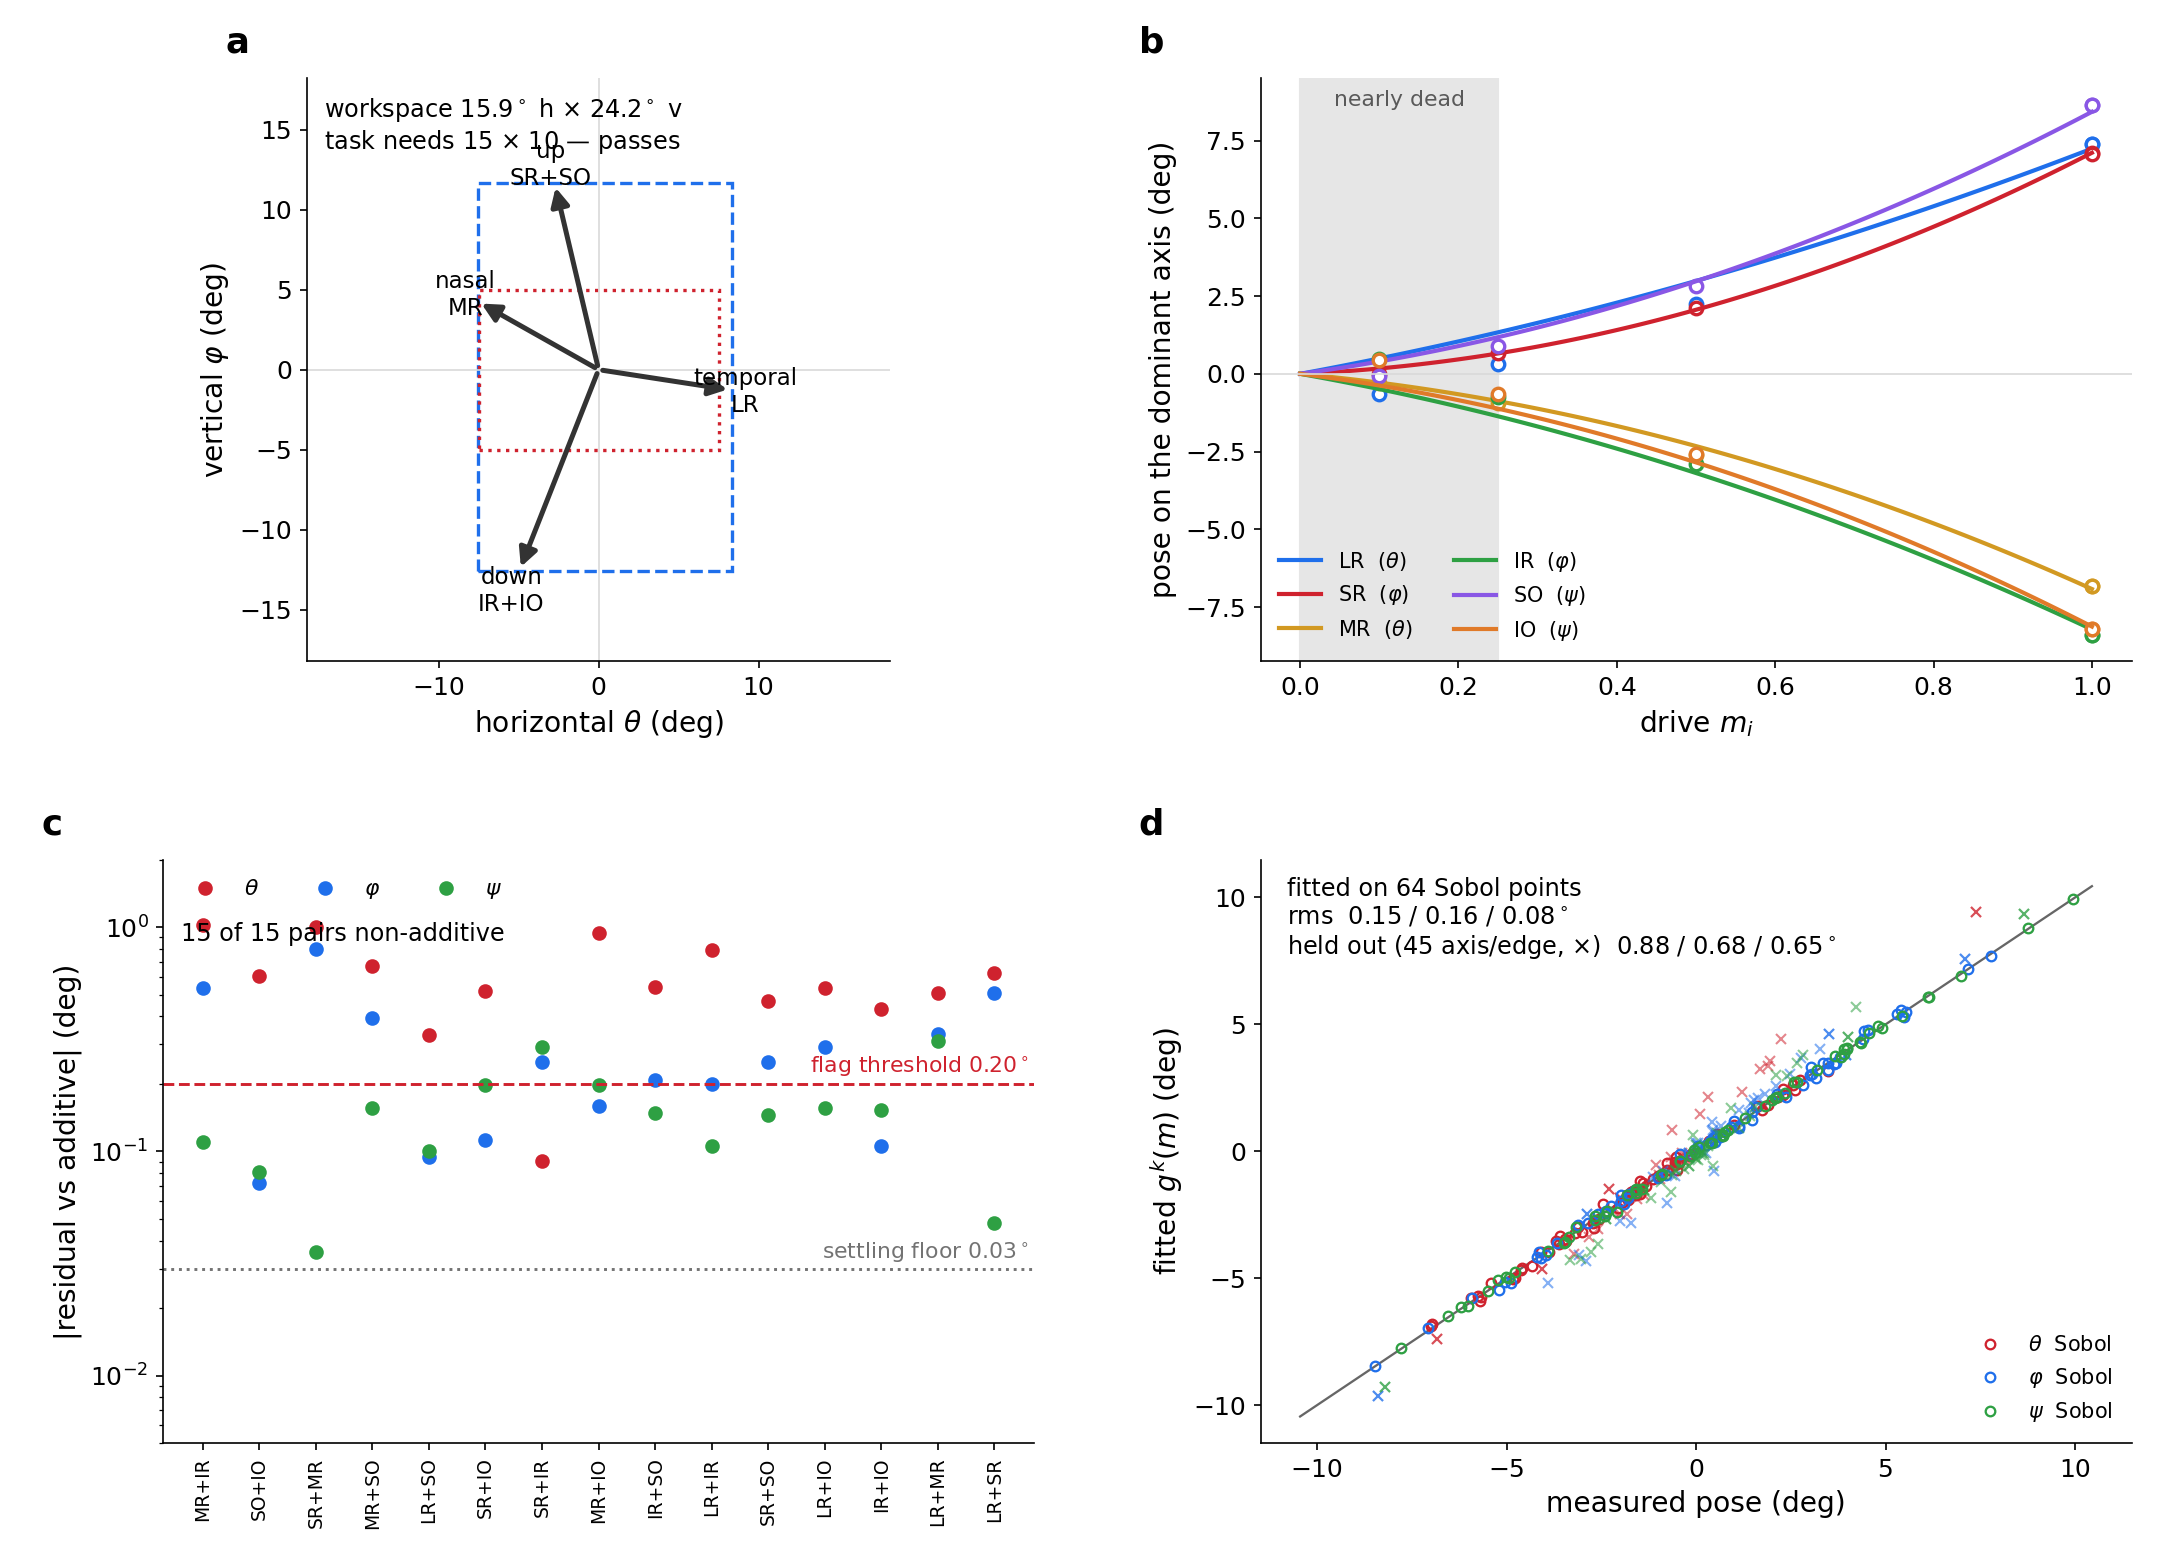
\includegraphics[width=\textwidth]{../figures/zebrafish/fig_eyeG_characterisation.png}
\caption*{\small \textbf{Eye G, characterised.} \textbf{(a)} Stage 0-lite: the four cardinal synergies driven open loop, each arrow the settled gaze excursion, the dashed box the workspace they span --- $15.9^{\circ}$ horizontal by $24.2^{\circ}$ vertical, against the $15/10$ the task needs. All four move the eye in the direction the insertions predict, which is what says the scanned anatomy is right. \textbf{(b)} Stage 1: the six marginals on each muscle's own dominant axis. The plant is nearly dead below $u\approx0.25$ and does most of its work in the upper half of the drive range, so a linearisation about rest is wrong in the direction that matters. \textbf{(c)} Stage 2a: the residual of each pair against its additive prediction, per angle, with the flag threshold and the numerical floor. All fifteen pairs interact, mostly in horizontal. \textbf{(d)} Stage 6d: the quadratic $g$ of \eqref{eq:quadratic} fitted over $64$ Sobol points in $[0,1]^6$, measured against fitted. Regenerate with \texttt{python Plexus/prototype/eye/fig\_eyeG\_charac.py}.}
\end{figure}

\paragraph{What it changes upstream}

Three things, all in section 5's notation. \textbf{Step 5} reads six non-negative drives rather than four, $\hat W^{\rm out}\in\mathbb{R}^{6\times N}$. \textbf{Step 7} becomes \eqref{eq:hammerstein}: one three-output static map and one $3\times3$ second-order block, in place of two independent single-input eyes; $g$, $C$ and $K$ are frozen buffers, as before, because the body is measured. And \textbf{step 8} gains a torsion penalty,

\begin{equation}
\mathcal{L}=\sum_{t}\big\|(\theta,\varphi)-(\theta^{\star},\varphi^{\star})\big\|_2
\;+\;\lambda_\psi\sum_{t}\psi(t)^{2},
\label{eq:loss-torsion}
\end{equation}

because six drives against two supervised angles leave a four-dimensional set of muscle patterns producing the same gaze, and the network will otherwise wander in it. This is not an arbitrary regulariser: real eyes resolve the same redundancy by holding torsion to a fixed function of gaze direction --- Donders' law, and its sharper form Listing's law --- and \eqref{eq:loss-torsion} is its simplest version. The three-dimensional treatment that makes it precise is Tweed and Vilis (1990) and Haslwanter (1995); adopting the full form later costs nothing, because the torsion coordinate is now in the model.

\paragraph{When an eye is good enough}

The same numbers for every eye, reported by the fit: the fraction of holds that settled, held-out rms per axis, the fraction of the command cube where the fitted map is monotone in each muscle's dominant axis, the reachable span per axis against the $15$ and $10$ degrees the task needs, the eigenvalues of $(C,K)$, and the size of the interaction terms against the marginals. Eye G passes the first four; its interaction terms are large, which is a property of the plant the controller must be trained through rather than a defect of the measurement.
\subsection*{5. Learning the controller}

The task is \textbf{supervised, not reinforcement}, and it is worth being explicit about why, because the instinct to reach for RL here is strong and wrong. In open loop the correct output is known in closed form at every timestep --- given the velocity stream, the target eye position is its integral. And the environment does not react to the agent: the dot moves the same way whatever the eye does. With no feedback loop and no unknown to explore, this is sequence-to-sequence regression trained by backpropagation through time. RL would recover the same gradient information with far more variance and no compensating benefit.

Closed loop does introduce a loop, but not a reason to change method: the eye is \texttt{gaze = integral of command}, which is differentiable, so one simply backpropagates through it. RL earns its place only where the objective stops being differentiable --- driving the MPM soft-body eye of \texttt{Plexus/prototype/eye} without backpropagating through the simulator, or choosing \emph{when} to make a catch-up saccade, which is a discrete decision rather than a continuous command. Smooth pursuit is regression; saccade timing is a policy.

\subsubsection*{5.1 How the recurrent models are trained}

Everything the controller learns comes from one scalar. Writing it in the symbols of section 4, with $(\theta_t,\varphi_t,\psi_t)$ the gaze the eye actually reaches and $(\theta^{\star}_t,\varphi^{\star}_t)$ the target eccentricity of step 0:

\begin{equation*}
\mathcal{L}\;=\;\frac{1}{T}\sum_{t=1}^{T}
\Big[\big(\theta_t-\theta^{\star}_t\big)^{2}
+\big(\varphi_t-\varphi^{\star}_t\big)^{2}\Big]
\;+\;\lambda_\psi\,\frac{1}{T}\sum_{t=1}^{T}\psi_t^{2},
\qquad \lambda_\psi=0.05
\end{equation*}

Note where the angles come from: $\theta,\varphi,\psi$ are the output of step 7, so the gradient reaches $\hat W$, $\hat W^{\mathrm{in}}$ and $\hat W^{\mathrm{out}}$ \emph{through} the eye. The eye's own coefficients are buffers rather than parameters and never move. The torsion term is the only part of the loss that is not a tracking error, and it is there because six drives against two supervised angles leaves a four-dimensional set of muscle patterns producing the same gaze; $\lambda_\psi$ picks one, and picking the untwisted one is Donders' law in its simplest form.

Three choices about how that loss is optimised are load-bearing.

The state starts at $v_i = 0$ for every neuron on every trial, never learned and never carried between trials. That is why the corpus is centre-started: $v_i = 0$ has to \emph{mean} "eye centred", so that the initial condition and the task agree. The loss is dense --- every timestep from $t=0$, not an endpoint --- which is what makes the teacher informative at every moment rather than only at the end.

The horizon grows during training, always as a prefix from $t=0$ rather than a sliding window:

\begin{center}\small
\begin{tabular}{lll}\toprule
epochs & horizon &  \\\midrule
0-62 & 120 steps & 2.0 s \\
63-124 & 240 steps & 4.0 s \\
125-186 & 360 steps & 6.0 s \\
187-249 & 480 steps & 8.0 s \\
\bottomrule\end{tabular}\end{center}

Each stage re-runs from $v_i = 0$ and truncates; there is no truncated BPTT and no carried state. Gradients flow through the whole unroll --- 480 sequential steps at the last stage, no detach --- with Adam at 2e-3 decayed by cosine to zero, gradient-norm clipping at 1.0, batch 128, so 29 updates per epoch and 7250 in total. The curriculum is not a refinement, it is the reason this trains: at the full 8 s horizon from a cold start the gradient of the integral vanishes, and beginning at 2 s makes the 8 s case reachable. It is the same device as \texttt{n\_steps\_schedule} in the heading-direction configs.

\textbf{What is trained, and what it reaches.} Two controllers, identical but for the eye between them and the width of the readout --- four synergy drives against the light eye, six muscle drives against the quadratic one:

\begin{center}\small
\begin{tabular}{lllll}\toprule
 & drives & corpus error & test sequence & mean torsion \\\midrule
\texttt{eyeG\_deep} & 6 muscles & \textbf{0.055°} & 0.10° & 0.03° \\
\texttt{eyeG\_light} & 4 synergies & 0.121° & 0.24° & 0.80° \\
\bottomrule\end{tabular}\end{center}

The corpus column is the 960-trial held-out set every controller in this document is scored on; the test sequence is 48 s of six regimes run continuously, which is six times the horizon either was trained at, and the growth between the two columns is open-loop drift accumulating exactly as section 2.3 says it must. Both beat the 0.185° the previous eye reached, and the six-muscle readout beats the four-synergy one twice over --- better tracking \emph{and} a twenty-fifth of the torsion --- because with six independent drives the controller can null the torsion against the position error instead of trading one for the other.

\paragraph{Regularisation: almost none, and one that is missing}

There is no weight decay, no penalty on $\hat W$, no spectral normalisation and no dropout. The only two terms that are not the tracking error are the torsion penalty above, which is a task constraint rather than a capacity one, and gradient-norm clipping at 1.0, which is a stability device.

That is defensible for capacity: train and validation error agree to the digit, so the network was never overfitting and a capacity regulariser would buy nothing. It would matter for \textbf{identifiability} rather than for fit --- many recurrent matrices integrate, and nothing here selects among them --- but in the constrained circuit that job is done by the sign lock of step 4, so the free-$\hat W$ controller is the wrong place to start adding priors.

What \emph{is} missing is a regulariser on the \textbf{drives}, and it is not cosmetic. The eye is characterised on $m\in[0,1]^{6}$ --- every hold in the protocol is at a level of 1 or below --- and above that the fitted quadratic simply extrapolates. The trained controllers do not stay inside:

\begin{center}\small
\begin{tabular}{lll}\toprule
 & max drive & fraction of the time above $m=1$ \\\midrule
\texttt{eyeG\_deep} & 1.67 & 12 \% \\
\texttt{eyeG\_light} & 4.16 & \textbf{77 \%} \\
\bottomrule\end{tabular}\end{center}

The readout is a softplus, which is unbounded above, and nothing in the loss objects. So the light controller spends three-quarters of its time in a regime where the eye model is pure extrapolation, and both leave it entirely on the step probe of section 5.2, where the command reaches 26 degrees against a 7-degree workspace. The real plant is known to behave badly there and not merely to be unmeasured: driving eye G at 1.5 times its working amplitude costs 6.4 \% of the globe's radius, takes peak muscle shortening from 26 \% to 74 \%, and makes two of the four cardinal synergies fail outright.

The fix is a hinge on the drive, $\lambda_m \sum_t \|[\mathbf{m}_t-1]_+\|^2$, which is free inside the characterised box and grows outside it. It should cost accuracy --- the pulse the network needs at a reversal is exactly what pushes $m$ past 1 --- and that trade is the point: a controller that tracks to 0.05 degrees by commanding a plant model outside its own validity is reporting a number about the extrapolation, not about the eye.

\subsubsection*{5.2 The controller rediscovered the pulse-step}

Watching the trained network drive the eye turns up something the training never asked for. Whenever the target reverses direction the \textbf{command} swings wildly while the \textbf{gaze} barely moves off the target: over the sharpest 3 \% of turns the gap between command and gaze grows 3.9 times, from 0.56 to 2.18 degrees, while the gaze error grows only 1.33 times, 0.098 to 0.130. The obvious reading is that the motor output has gone unstable and the eye's own smoothing rescues it.

It is not instability. It is the eye's inverse, and the inverse has a closed form, so the claim is falsifiable. The eye of step 7 is

\begin{equation*}
\ddot{\mathbf{x}} + C\,\dot{\mathbf{x}} + K\,\mathbf{x} \;=\; K\,\mathbf{x}_{\infty}
\end{equation*}

and rearranging for the command that would place the gaze exactly on a wanted trajectory $\mathbf{x}^{\star}(t)$ gives

\begin{equation*}
\mathbf{x}_{\infty}^{\star}
\;=\;\mathbf{x}^{\star}
\;+\;K^{-1}C\,\dot{\mathbf{x}}^{\star}
\;+\;K^{-1}\ddot{\mathbf{x}}^{\star}
\end{equation*}

Read it in plain terms: to hold the eye somewhere, ask for that place; to move it, ask for somewhere \emph{further}, in proportion to how fast you want to go; and to start or stop the movement, add a term proportional to the acceleration. A step in $\mathbf{x}^{\star}$ makes the velocity term a pulse and the acceleration term a doublet, and what is left afterwards is the step. \textbf{That is Robinson's pulse-step}, falling out of the algebra rather than being designed in --- the same pulse-step section 4.1 credits Robinson (1964, 1981) with, as the command that inverts the linear eye. Nothing in this model was told about it.

\begin{figure}[H]\centering
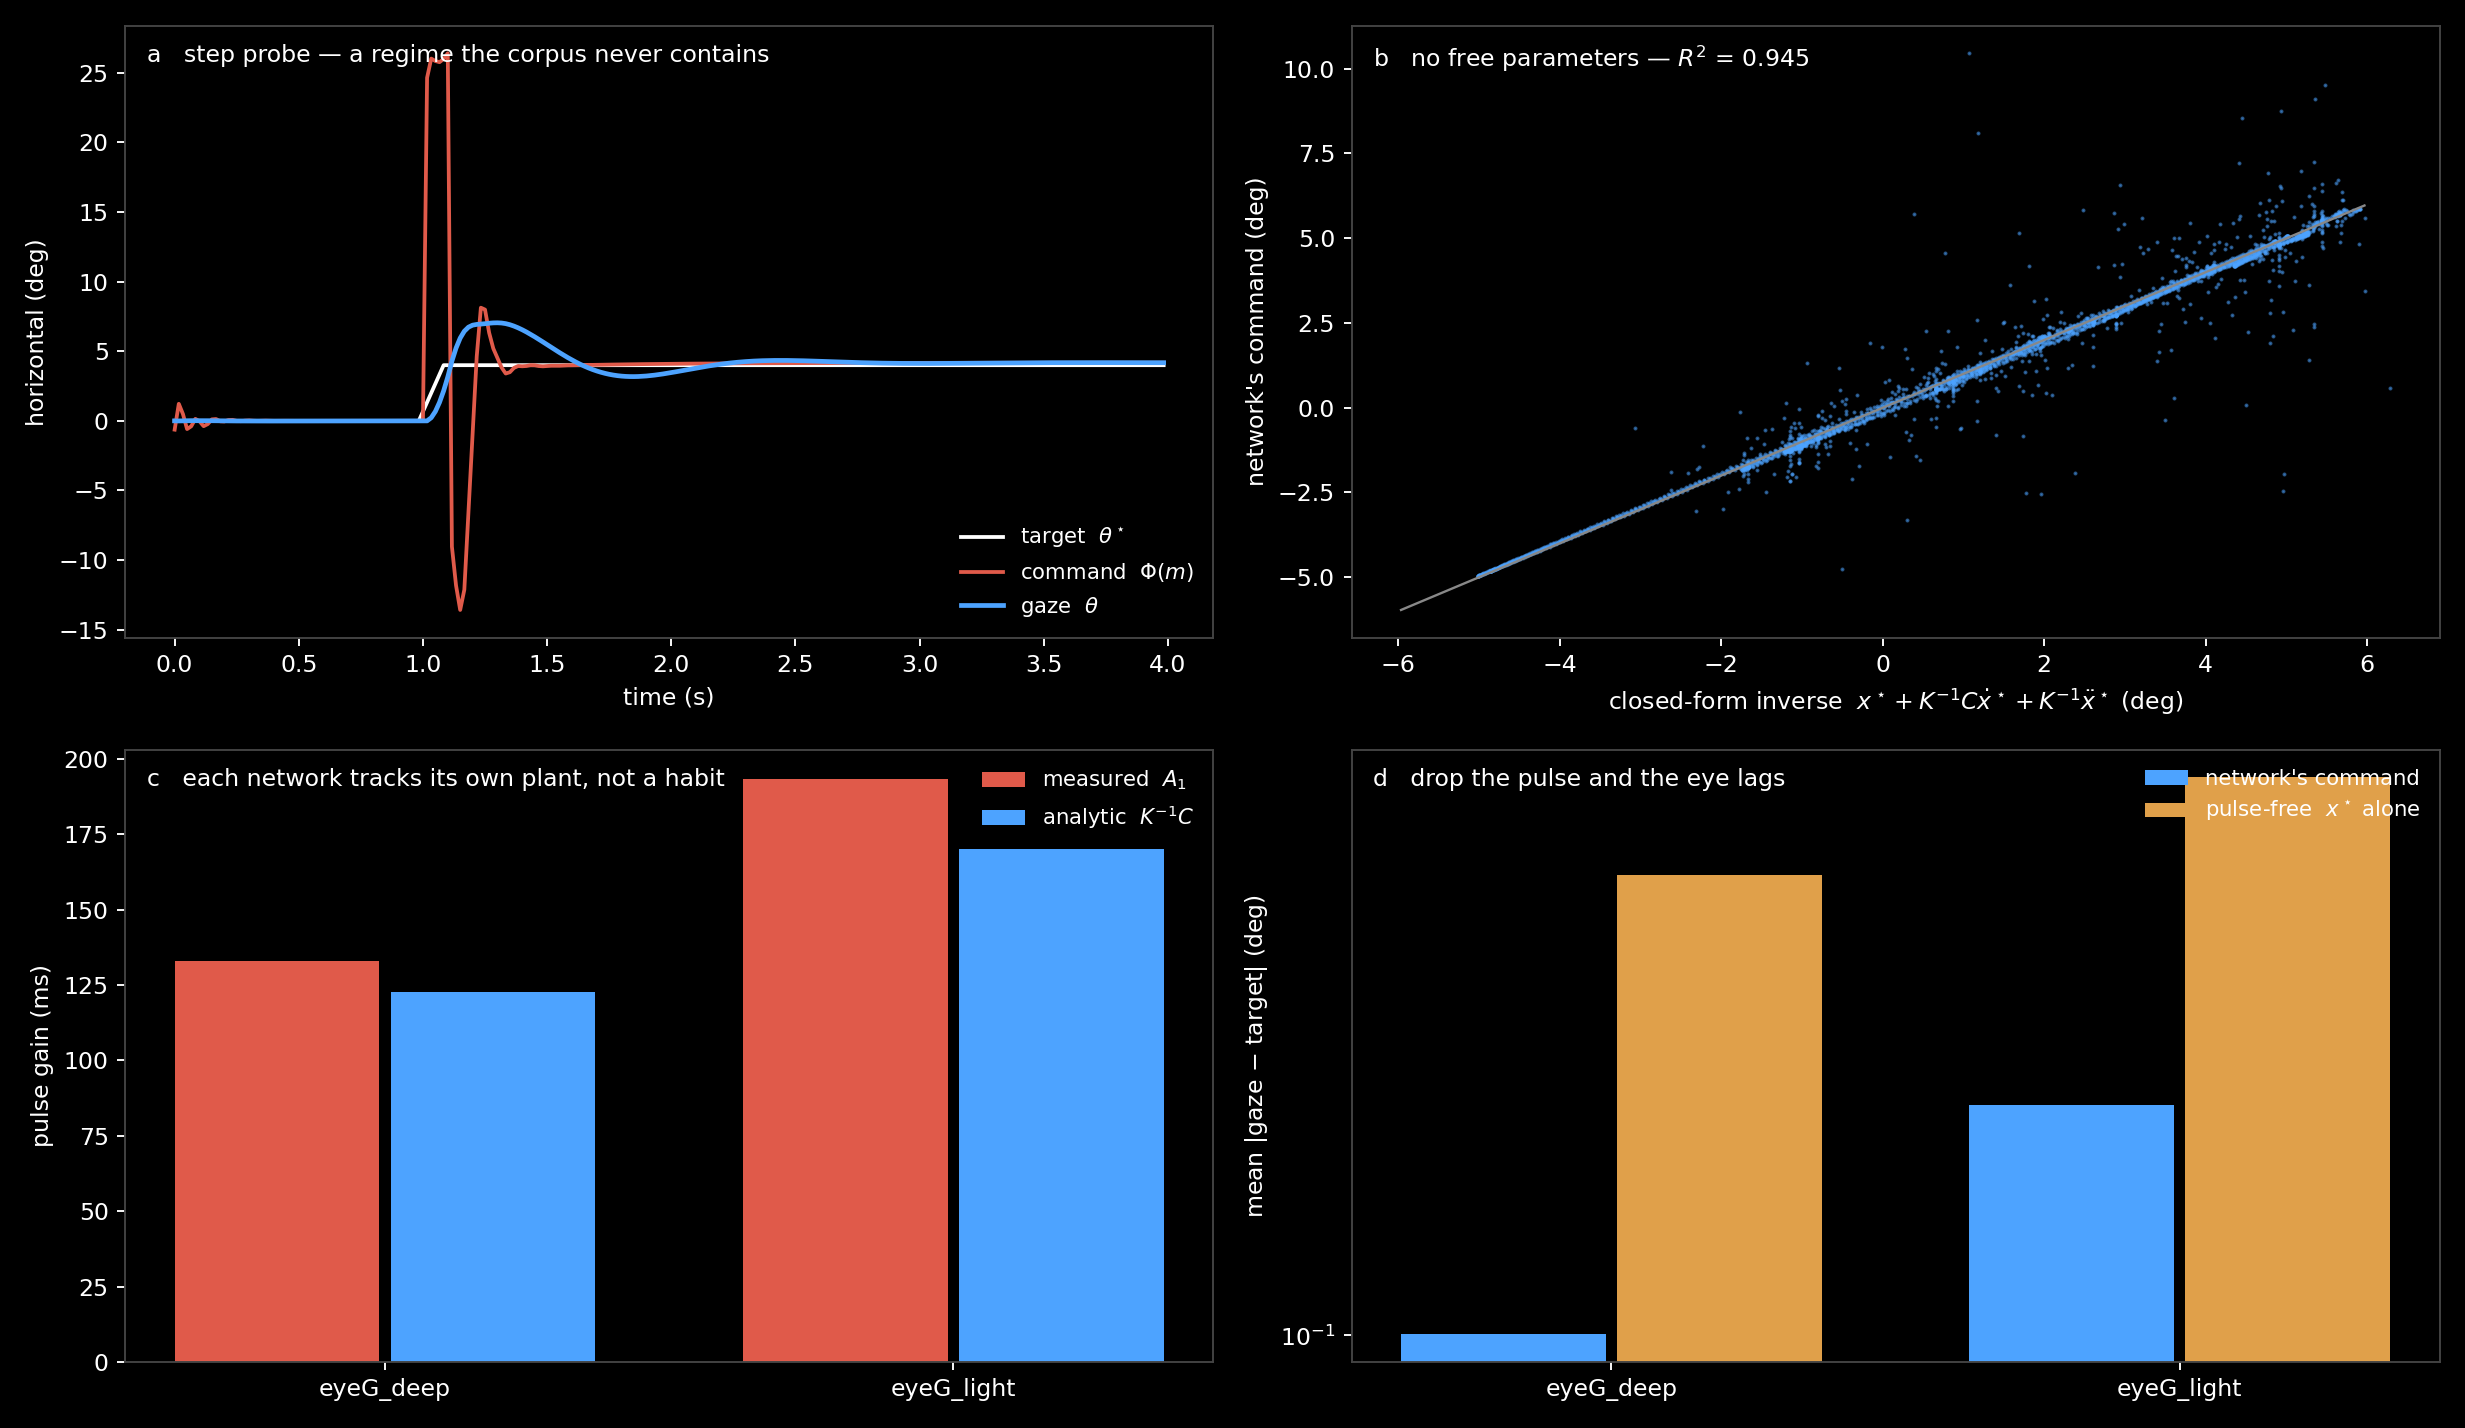
\includegraphics[width=\textwidth]{../figures/zebrafish/fig_pulse_step.png}
\caption*{\small \textbf{The controller learned the eye's inverse, not a tracking habit.} \textbf{(a)} A step probe: the target steps 4° and holds. The corpus contains no steps --- it is splines at three speeds --- so this regime is new to the network. The command goes to $+26°$, brakes to $-14°$, then settles on the $+4°$ step, while the gaze rises smoothly to the target: accelerate, brake, hold. The doublet is the $K^{-1}\ddot x^{\star}$ term and the offset that survives it is $x^{\star}$. \textbf{(b)} The network's command against the closed-form inverse above, evaluated with the eye's own $K$ and $C$ and \textbf{no free parameters}: $R^2 = 0.945$. Fitting $A_0, A_1, A_2$ freely reaches only 0.952, so the analytic matrices cost essentially nothing. \textbf{(c)} The velocity gain $A_1$ of each network against its own $K^{-1}C$. The two eyes differ by 46 \% in measured pulse gain (133 against 193 ms) and each matches its own plant; a pulse that was a habit of the architecture or of the corpus would be the same in both. \textbf{(d)} Necessity: drive each eye with the pulse-free command $x^{\star}$ and the tracking error rises 5.9$\times$ on the deep eye (0.101 $\rightarrow$ 0.592°) and 3.5$\times$ on the light one. Regenerate with \texttt{python fig\_pulse\_step.py} in \texttt{prototype/dot\_tracking}.}
\end{figure}

\textbf{Why "learned" rather than "built in".} Four things have to be true at once, and each is measured in the figure.

\emph{The shape is not memorised.} The corpus is splines at three speeds and contains no steps at all; the step probe of panel (a) is a regime the network has never been in, and it produces the pulse-step there.

\emph{The coefficients are the plant's.} Regressing the command freely on the target and its first two derivatives, $\mathbf{m}_{\rm cmd}\approx A_0\mathbf{x}^{\star} + A_1\dot{\mathbf{x}}^{\star} + A_2\ddot{\mathbf{x}}^{\star}$, reaches $R^2 = 0.952$; \emph{replacing} the fitted $A_1, A_2$ with the analytic $K^{-1}C$ and $K^{-1}$ --- no free parameters at all --- still reaches 0.945. The network's velocity gain is 133 ms against the plant's 123. Note the regressor is the \textbf{target}, not the achieved gaze: regressing on the gaze would be circular, since the equation above makes that an identity for any command whatsoever.

\emph{It is this eye's inverse, not an eye's.} The deep and light controllers were trained identically on the same corpus and differ only in the eye between them. Their pulse gains differ by 46 \%, 133 against 193 ms, and each tracks its own $K^{-1}C$, 123 against 170. An architectural habit would not know which plant it was attached to.

\emph{The loss had no alternative.} Driving the same eye with the pulse-free command --- just $\mathbf{x}^{\star}$, no velocity or acceleration term --- costs a factor of 5.9 in tracking error on the deep eye and 3.5 on the light one. The pulse is not decoration the optimiser could have skipped.

Two structural points make the result sharper. Nothing in the architecture supplies $\dot{\mathbf{x}}^{\star}$ or $\ddot{\mathbf{x}}^{\star}$: the readout is a static map of the rates, so the velocity term has to come from the input --- which \emph{is} the target velocity, scaled --- while the position term must be integrated out of it and the acceleration term differentiated out of it, both by the recurrent dynamics alone. And $K$ and $C$ appear nowhere in the loss; they are buffers inside a frozen eye the gradient passes \emph{through}. The controller inferred them from the only thing it was ever shown, which is how far the gaze ended up from the target.

One last thing worth naming. The recurrent matrix is initialised at exactly zero and every per-neuron time constant is free to grow, so the network could in principle have put this in its membranes. It did not: what it built is an inverse model of the body it is attached to, from a velocity stream and a squared error at the far end of that body, and nothing else.

\subsection*{6. Progress, 11 August 2026}

Opened the branch \texttt{feat/oculomotor} and put the zebrafish configs back under version control --- 254 of them had been absent from every worktree since the \texttt{config/zebrafish} bind-mount was commented out of \texttt{devcontainer.json}, which left no figure script able to resolve a run config. Traced how the 917-cell heading-direction circuit was actually built (the colleagues' pickle, not the neuPrint query the filenames suggest) and wrote that up as \texttt{HOWTO\_add\_oculomotor\_circuit.md}, since the same five inputs are needed again here. Read the new \texttt{Oculomotor\_sortedData\_081126.pkl}: 2949 cells, 42 types, 5 keys, no per-cell ordering variable; confirmed its matrix orientation empirically rather than assuming it. Selected the sub-circuit in two steps --- first the 244-cell INTG/AMN/AIN core, then 285 cells once AF5 was added, which gave the pool the afferent stage it had been missing. Introduced \texttt{CellTypeSpec} so each type's pool, Dale sign, L/R split and role live in the config where they can be reviewed, rather than in hardcoded prefix tuples inside the loader. Rendered the two-panel connectivity figure above, and wrote this note.

Nothing has been trained, and no connectome CSVs exist yet. The five decisions below are what stand between this document and a first run.

\subsection*{7. What has to be decided next}

\begin{enumerate}\setlength{\itemsep}{1pt}
  \item \textbf{The AF5 combination rule} (\S{}1.3) --- AND, OR or XOR. Blocks the input model.
  \item \textbf{Whether \texttt{OMN} joins the pool} (\S{}1.5) --- decides whether \texttt{AIN} -> medial rectus is one synapse or two.
  \item \textbf{Whether \texttt{Burst\_*} joins the pool} (\S{}1.6) --- decides whether the saccadic regime has an anatomical input or an injected one.
  \item \textbf{The readout convention} --- scalar eye position, or innervation of the \texttt{LR}/\texttt{MR} pair coupled to the soft-body eye.
  \item \textbf{The target leak \texttt{xi\_tau\_s}} --- a free parameter, or the quantity to be fitted against recorded eye position.
\end{enumerate}

\subsection*{Appendix A. Which simulator, now that there are meshes}

\textbf{The question.} A colleague is segmenting the six extraocular muscles and the globe from imaging, so for the first time we will have real anatomy rather than a hand-built approximation of it. Something has to consume those meshes and turn them into a moving eye. The realistic candidates are MuJoCo, the material-point simulator already in \texttt{Plexus/prototype/eye}, and a reimplementation of that simulator on NVIDIA's Warp.

\textbf{The answer, first.} Keep the material-point simulator. MuJoCo is faster, more mature and --- importantly --- already differentiable, which would remove the need for the fitted surrogate of section 4.2 entirely. But it cannot represent tissue that both deforms a lot and has different stiffness in different places, and that is precisely what a per-muscle segmentation is for. The medium-term move is to port the material-point simulator to Warp, which keeps the physics and adds the differentiability.

\textbf{What the choice turns on.} Not speed, and not accuracy in the abstract. It turns on what a segmented mesh is \emph{for}. If the meshes are only there to fix where each muscle attaches and which way it pulls, a rigid globe with six cables wrapped around it uses all of that and runs a hundred times faster. If the meshes are there because the muscle belly, the tendon and the sclera behave differently and deform substantially while pulling, then the mesh is tissue, and only a simulator that carries material properties through the volume can use it. The second is the stated intent, so it decides the question.

\begin{center}\small
\begin{tabularx}{\textwidth}{>{\raggedright\arraybackslash}X>{\raggedright\arraybackslash}X>{\raggedright\arraybackslash}X>{\raggedright\arraybackslash}X>{\raggedright\arraybackslash}X>{\raggedright\arraybackslash}X}\toprule
 & mesh becomes & different materials & large deformation & gradients & speed \\\midrule
MuJoCo, rigid globe + cable muscles & attachment points, wrap surfaces & not applicable & not applicable & yes (MJX / MuJoCo-Warp) & very fast \\
MuJoCo, deformable objects (\texttt{flex}) & tetrahedral volume & one per flex, or per edge & \textbf{no --- small strain only} & yes & slow at high resolution \\
our material-point simulator & particles filling the volume & per particle & yes & \textbf{no} & slow \\
material-point on Warp & particles filling the volume & per particle & yes & yes, and batched & fast \\
\bottomrule\end{tabularx}\end{center}

\textbf{MuJoCo with a rigid globe} is the strongest option we are turning down, so it is worth being clear about what is being given up. It has a muscle model built in --- the standard force-length-velocity relation, the same curve our thirty single-muscle holds exist to measure --- so stage 1 of the protocol would simply not be needed. Its cables can be routed through wrap surfaces, which is a direct implementation of the connective-tissue pulleys Demer and colleagues established are real, and which eye D imitated with a sleeve constraint. And MuJoCo-Warp reports speedups of seventy to a hundred times with gradients available, so the eye could sit inside the training loop and be backpropagated through, rather than being replaced by a fitted stand-in. The cost is that the globe is rigid and the muscles are one-dimensional cables: the segmentation contributes geometry and nothing else, and every distinction between sclera, tendon and muscle belly is discarded on import.

\textbf{MuJoCo's deformable bodies} are the obvious way to keep the tissue, and they do not work here. First a word on the terms, because they mislead: a MuJoCo \emph{body} is a rigid element of a kinematic tree and has no stiffness at all. Deformable objects are a separate element, \texttt{flex}, added in MuJoCo 3.0. MuJoCo is a rigid-body contact engine with deformation built on top, which is not a criticism --- it is what it was designed for --- but it is why continuum tissue sits awkwardly in it.

Two limits then apply. A flex carries \textbf{one} Young's modulus and one Poisson ratio for the whole object, so sclera, tendon and bone cap --- 300, 9 and 40 in eye A --- need three separate flexes fastened together, and joining elastic objects is reported to work only by giving each its own body. There is a partial escape: a flex is a mesh of edges, and edges carry stiffness and damping individually, so stiffness \emph{can} be varied inside one flex at the edge level. But that means abandoning the continuum parameters and calibrating springs instead, which for a segmentation whose whole point is "this region is tendon and that region is sclera" is a downgrade rather than a solution.

More decisively, the deformation model is only valid for \emph{small} strains, and warns that tetrahedra can invert under large load. A rectus muscle shortening by a third is not a small strain. That is a limitation of the method rather than of the implementation, so a newer version will not fix it --- and it is consistent with the accuracy users report in large-deflection tests, where a beam expected to deflect 2.15 m settled at about 0.26 m. The rest of the implementation is improving quickly, for what it is worth: the solid elasticity model has moved from a plugin into the engine, and flex stiffness is now solved implicitly alongside contact rather than added as an external force.

\textbf{The material-point method} has the opposite profile, and it is the reason the prototype uses it. Material properties are carried by the particles, so every particle can differ and a mesh can be filled directly without being converted to tetrahedra first; and large deformation is the case the method was invented for, with no mesh to tangle. What it costs is everything section 4.2 already documents: the grid scatter overwrites its own memory, so the simulator cannot be differentiated, and it is far too slow to sit inside seven thousand gradient updates. That is the entire reason the surrogate exists.

\textbf{The material-point method on Warp} removes that cost without giving up anything above. Warp is a way of writing GPU code in Python with automatic differentiation built in, and material-point solvers written on it are public: \texttt{warp-mpm}, used in the PhysGaussian work, interoperates directly with PyTorch; GeoWarp is a differentiable implicit solver built specifically to fit material parameters by gradient descent; Rewarped runs many deformable simulations in parallel and returns gradients for all of them, which is the form training actually needs, since a batch is a hundred and twenty-eight trials at once. Per-particle stiffness is the natural representation there --- an array indexed by particle, with the gradient flowing back into it. Two honest caveats: this is a port rather than a setting, and GeoWarp demonstrates fitting one scalar parameter and describes spatially varying parameters as a generalisation rather than a result.

\textbf{The plan, and the measurement that would change it.} Near term, nothing changes: the material-point eye and the fitted surrogate of section 4.2, which work today and depend on no port. Medium term, port to Warp and put the eye itself in the training loop. The surrogate is not wasted either way --- a differentiable simulator still has to be shown to reproduce the measured static map and mechanics, and the protocol's holds are exactly that test.

The one measurement that would overturn this is cheap. Build the MuJoCo version --- rigid globe, six cables through wrap surfaces, the built-in muscle model --- and run stage 0 and stage 1 on it. If it reproduces the measured span and the six single-muscle curves to within the accuracy the tracking task is scored at, then the deforming tissue is not buying anything the task can see, and we should take the hundredfold speedup and the free gradients. That is a day's work and it is worth doing before the port, not after.
\end{document}
